%20 min preso!
\documentclass[aspectratio=169,xcolor=table,english]{beamer}
\usepackage{beamerthemesplit}
\usepackage{wrapfig}
\usetheme{SPbGU}
\usepackage{pdfpages}
\usepackage{amsmath}
\usepackage{mathtools}
\usepackage{cmap}
\usepackage{subcaption}
\usepackage[utf8]{inputenc}
\usepackage[T1, T2A]{fontenc}
\usepackage[]{babel}
\usepackage{indentfirst}
\usepackage{amsmath}
\usepackage{tikz}
\usepackage{multirow}
\usepackage[noend]{algpseudocode}
\usepackage{algorithm}
\usepackage{algorithmicx}
\usepackage{fancyvrb}
\usetikzlibrary{calc}
\usetikzlibrary{shapes,arrows}
\usetikzlibrary{arrows,automata}
\usetikzlibrary{positioning}
\usetikzlibrary{fit}

\usepackage{kbordermatrix} % include package @ document preamble
\renewcommand{\kbldelim}{(} % change default array delimiters to parentheses
\renewcommand{\kbrdelim}{)}

\newcommand\mca{\multicolumn{1}{c}{\cellcolor{red}\textbf{\{a\}}}}
\newcommand\mcb{\multicolumn{1}{c}{\cellcolor{red}\textbf{\{b\}}}}

\usepackage{tabularx}
\newcolumntype{Y}{>{\raggedleft\arraybackslash}X}

\renewcommand{\thealgorithm}{}

\newtheorem{mytheorem}{Theorem}
\renewcommand{\thealgorithm}{}

\newcommand{\tikzmark}[1]{\tikz[overlay,remember picture] \node (#1) {};}
\def\Put(#1,#2)#3{\leavevmode\makebox(0,0){\put(#1,#2){#3}}}

\newcommand{\ltz}{$< 1$}

\tikzset{
    state/.style={
           rectangle,
           rounded corners,
           draw=black, very thick,
           minimum height=2em,
           inner sep=2pt,
           text centered,
           },
}

\beamertemplatenavigationsymbolsempty

\title[Tensor CFPQ GPGPU]{Реализация алгоритма поиска путей в графовых базах данных через тензорное произведение на GPGPU}
% \subtitle[YaccConstructor]{Parsing techniques for graph analysis}
% То, что в квадратных скобках, отображается в левом нижнем углу.
\institute[СПбГУ]{
Программная инженерия
}

% То, что в квадратных скобках, отображается в левом нижнем углу (прикольно).
\author[Егор Орачев]{Орачев Егор Станиславович, 17.Б11-мм \\Научный руководитель: доцент кафедры информатики, к.ф.-м.н. С.В. Григорьев\\Рецензент: разработчик биоинформатического ПО, ЗАО “БИОКАД” А.С. Хорошев}
\date{29 апреля 2021}


\begin{document}
{
\begin{frame}[fragile]
  \begin{table}
  \centering
  \begin{tabularx}{\linewidth}{YcX}
    %
\includegraphics[height=1.5cm]{pictures/jetbrainsResearch.pdf} \hfill
    %& 
    \begin{minipage}[t]{1.0\textwidth}\center 
    %\vspace{-1cm} 
    Санкт-Петербургский Государственный университет
      \end{minipage}
    %& \hfill 
\includegraphics[height=1.5cm]{pictures/SPbGU_Logo.png}
  \end{tabularx}
  \end{table}
  \titlepage
\end{frame}
}

\begin{frame}[fragile] \frametitle{Введение}
    \begin{minipage}[m]{0.6\linewidth}
        \begin{figure}
            \centering
            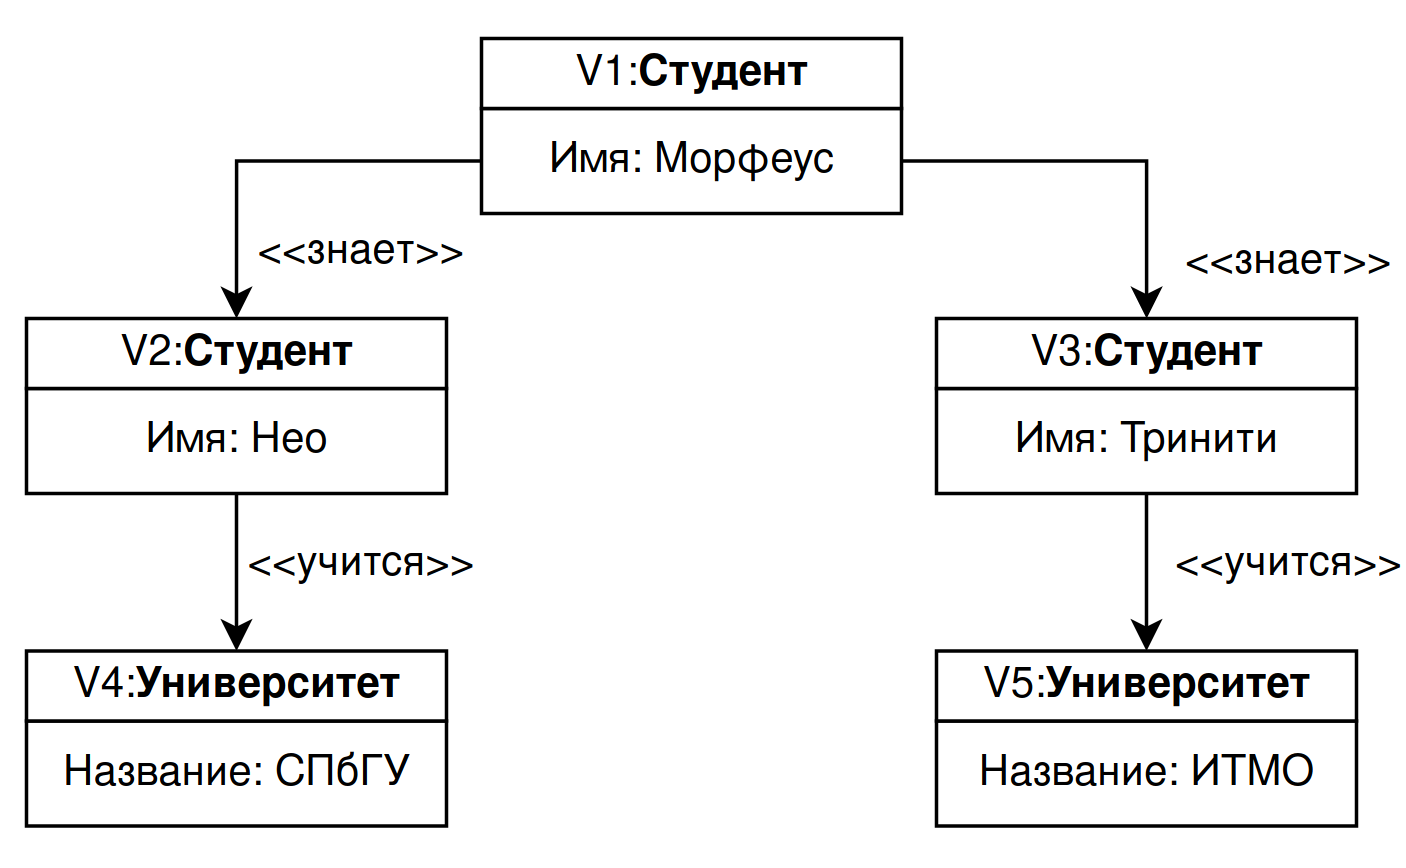
\includegraphics[width=\textwidth]{figures/db_example.png}
            \caption{Пример графовой БД}
            \label{fig:architecture}
        \end{figure}
    \end{minipage}\hfill
    \begin{minipage}[m]{0.4\linewidth}
        \begin{itemize}
            \item Графовая модель данных
            \item Графовые базы данных
            \item Граф программы, потока управления, данных и т.д
            \item Запрос к графовой БД: ограничение на пути
        \end{itemize}
    \end{minipage}
\end{frame}

\begin{frame}[fragile] \frametitle{Запросы с КС ограничениями}
    \begin{minipage}[m]{0.45\linewidth}
        \begin{figure}
            \centering
            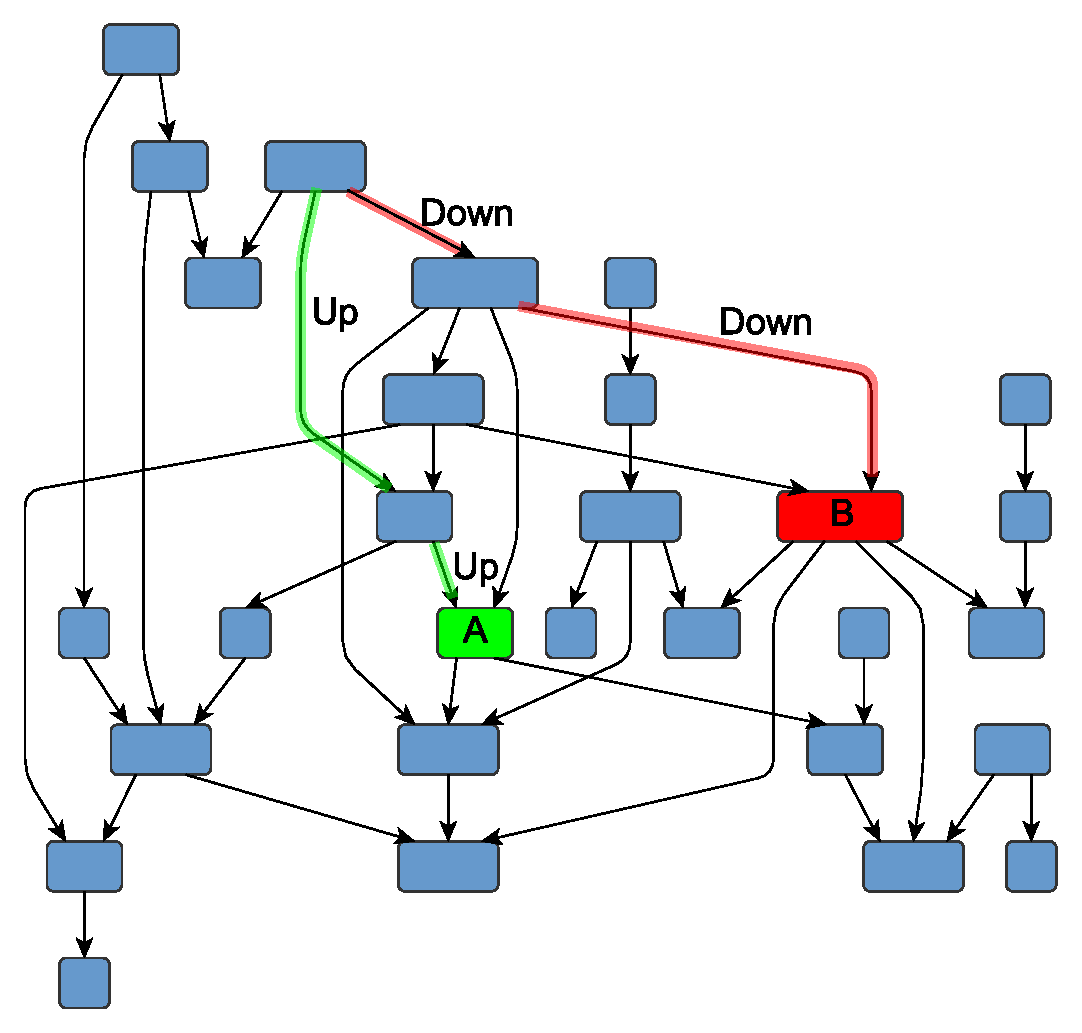
\includegraphics[width=\textwidth]{pictures/hierarchical.pdf}
            \caption{Пример графа}
        \end{figure}
    \end{minipage}\hfill
    \begin{minipage}[m]{0.5\linewidth}
        \begin{itemize}
            \item Мотивация: навигация в графе
            \item Пример: находятся ли вершины A и B на одном уровне иерархии?
            \item Применение: анализ RDF данных, биоинформатика, статический анализ кода
            \item Проблема: отсутствие поддержки КС запросов как в современных СУБД, так и в отдельных инструментах
        \end{itemize}
  \end{minipage}
\end{frame}

\begin{frame}[fragile] \frametitle{Алгоритмы поиска путей с КС ограничениями}
    \begin{itemize}
        \item На основе линейной алгебры:
        {
        \begin{itemize}
            \item Алгоритм Рустама Азимова
            \item \textbf{Алгоритм на основе тензорного произведения}\footnote{Context-Free Path Querying by Kronecker Product, Egor Orachev, Ilya Epelbaum, Rustam  Azimov, Semyon Grigorev. Дата обращения: 9.04.2021. Ссылка на статью: \url{https://link.springer.com/chapter/10.1007/978-3-030-54832-2\_6}}
        \end{itemize}
        }
        \item Операции: матричное умножение, поэлементное сложение, произведение Кронекера и т.д. в булевом полукольце
        \item Структура матриц: разреженная
        \item Для эффективной реализации требуется библиотека примитивов разреженной булевой линейной алгебры на GPGPU
    \end{itemize}
\end{frame}

\begin{frame}[fragile] \frametitle{Цель и задачи}
    \textbf{Целью} данной работы является реализация алгоритма поиска путей в графовых базах данных через тензорное произведение на GPGPU.
    
    \textbf{Задачи}:
    \begin{itemize}
        \item Разработка архитектуры библиотеки примитивов разреженной линейной булевой алгебры для вычислений на GPGPU
        \item Реализация библиотеки в соответствии с разработанной архитектурой
        \item Реализация алгоритма поиска путей с КС ограничениями через тензорное произведение с использованием разработанной библиотеки
        \item Экспериментальное исследование полученных результатов
    \end{itemize}
\end{frame}

\begin{frame}[fragile] \frametitle{Требования к библиотеке}
    \begin{itemize}
        \item Поддержка вычислений на Cuda-устройстве
        \item Поддержка вычислений на CPU
        \item C-совместимый API для работы с библиотекой
        \item Python-пакет для работы с примитивами и операциями библиотеки в управляемой высокоуровневой среде языка Python
        \item Поддержка логирования, функций для отладки и прототипирования конечных пользовательских алгоритмов
    \end{itemize}
\end{frame}

\begin{frame}[fragile] \frametitle{Архитектура библиотеки}
    \begin{center}
    \begin{minipage}[m]{\linewidth}
        \begin{figure}
            \centering
            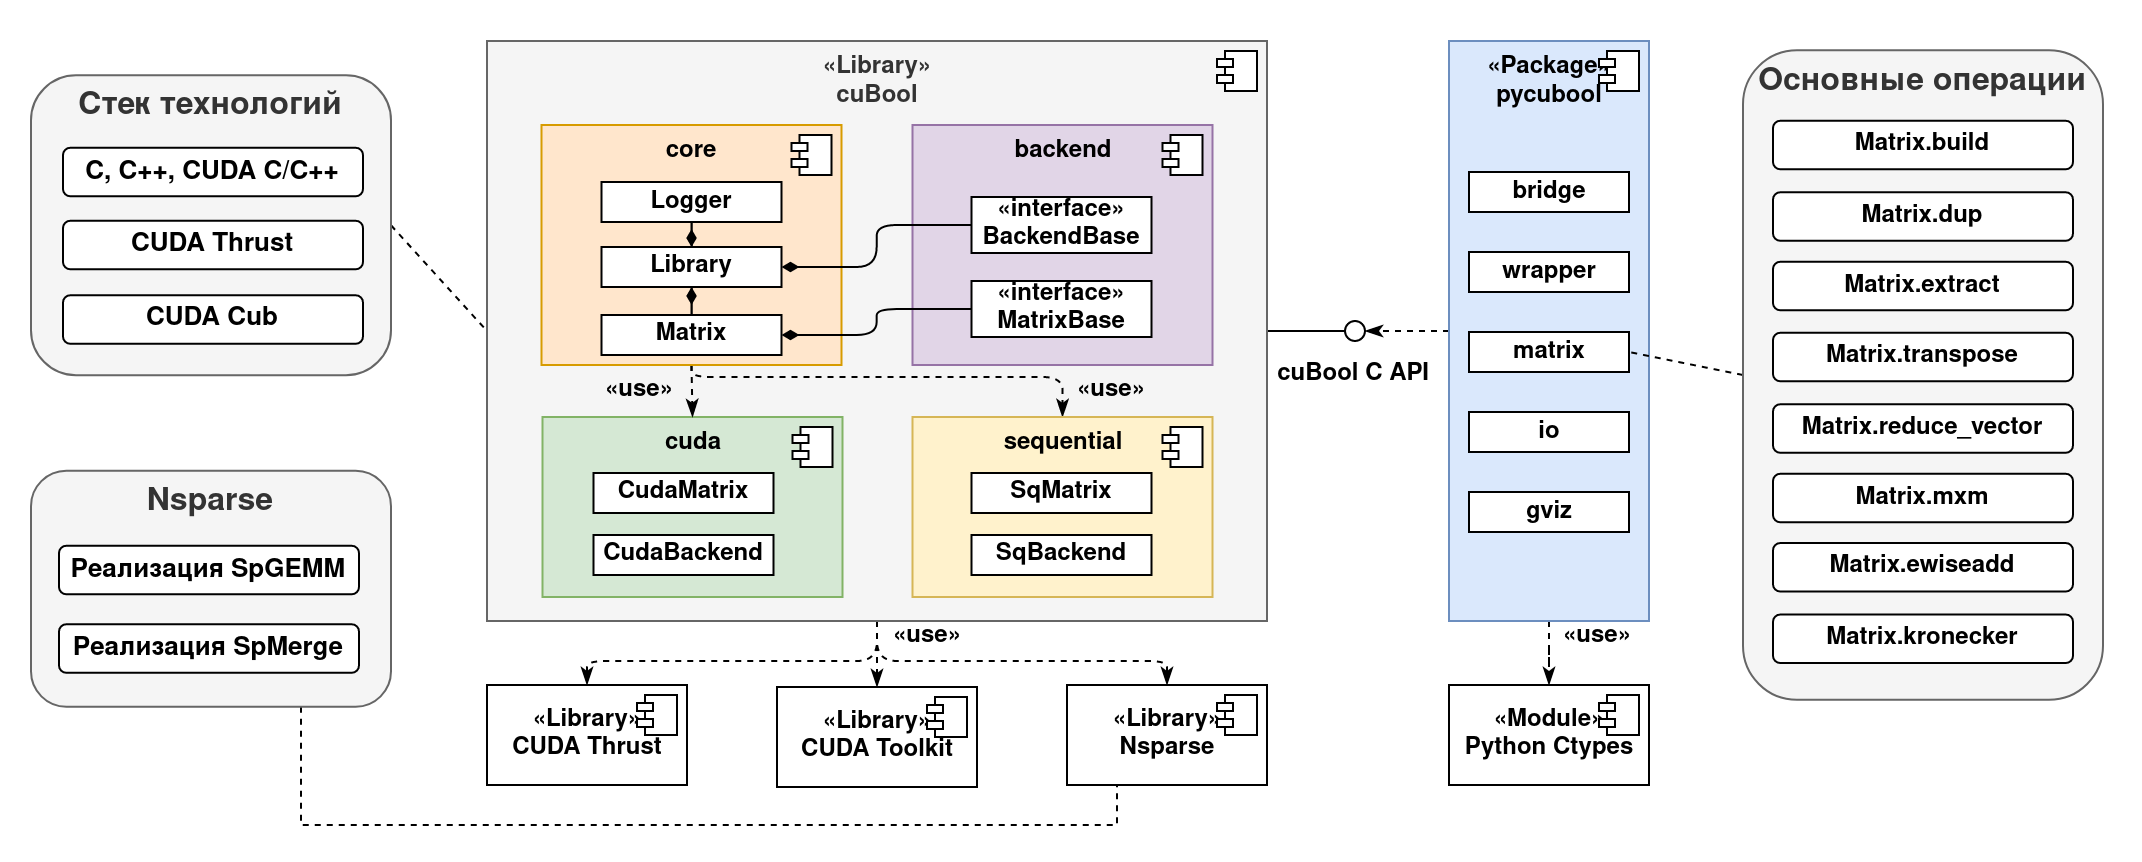
\includegraphics[width=0.4\textwidth]{figures/library_architecture.png}
            \caption{Архитектура разработанной библиотеки}
        \end{figure}
    \end{minipage}\hfill    
    \end{center}
\end{frame}

\begin{frame}[fragile] \frametitle{Последовательность обработки операций}
    \begin{center}
    \begin{minipage}[m]{0.85\linewidth}
        \begin{figure}
            \centering
            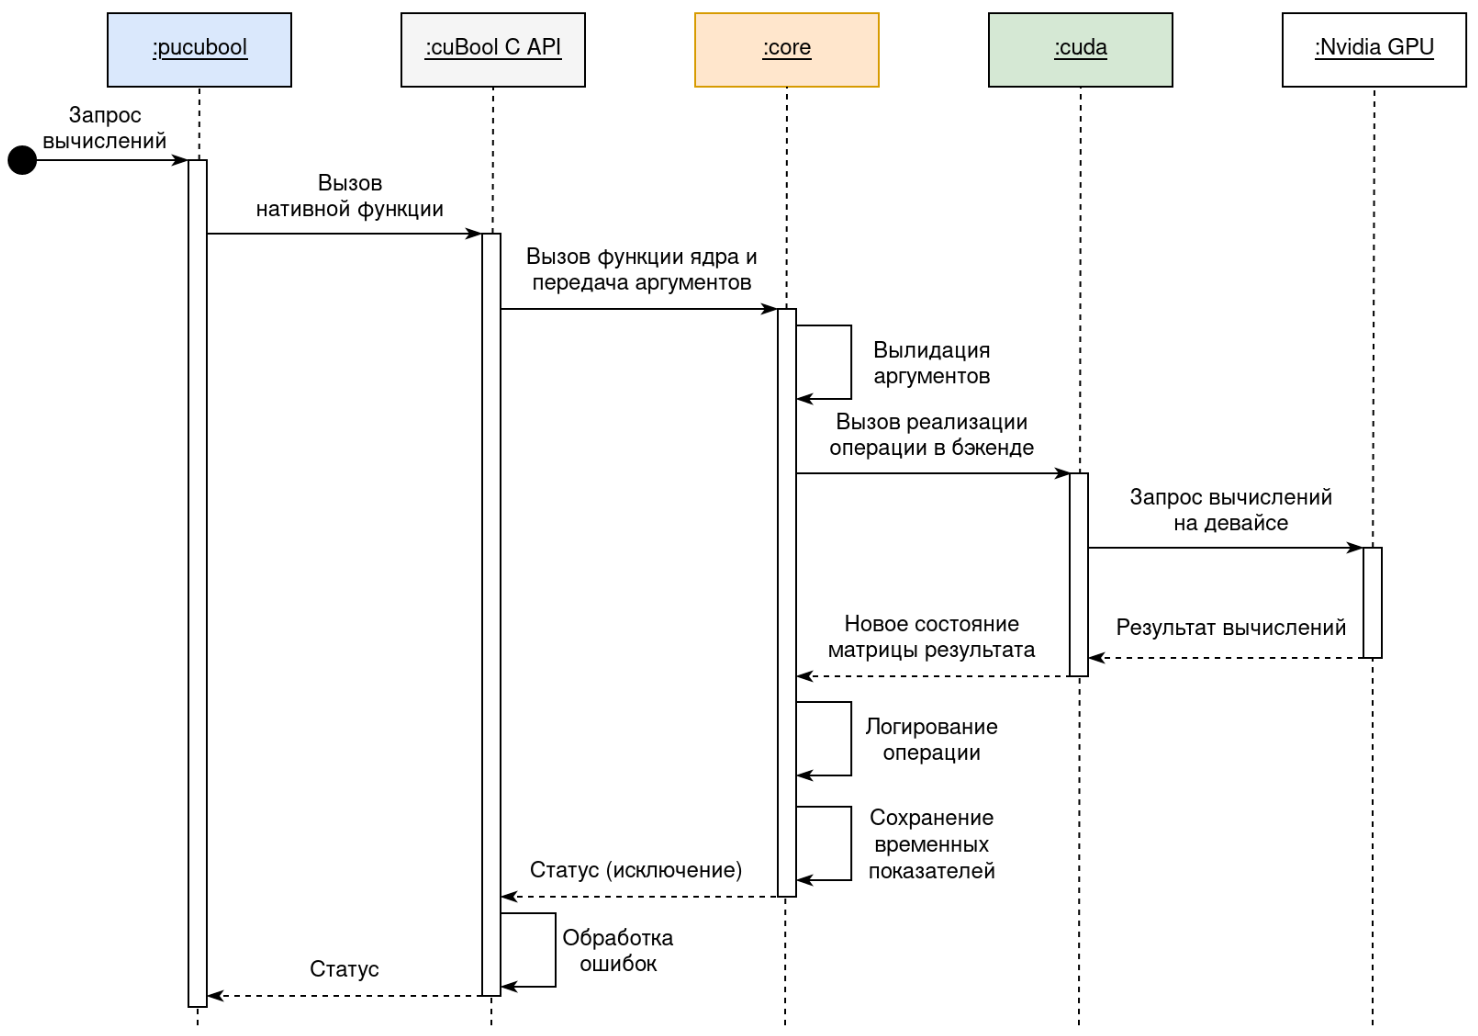
\includegraphics[width=0.65\textwidth]{figures/library_call_flow.png}
            \caption{Последовательность выполнения вычислительной матричной операции на Nvidia GPU с использованием pycubool}
        \end{figure}
    \end{minipage}\hfill    
    \end{center}
\end{frame}

\begin{frame}[fragile] \frametitle{Детали реализации}
    \begin{itemize}
        \item C, C++, CUDA C/C++, Python
        \item Разреженная матрица булевых значений хранится формате CSR
        \item Размер в памяти $\textit{sizeof(unsigned int)} * (\textit{rows} + 1 + \textit{nvals})$
        \item Операции: 
        {
        \begin{itemize}
            \item Умножение
            \item Поэлементное сложение
            \item Произведение Кронекера
            \item Транспонирование
            \item Редуцирование к вектор-столбцу
            \item Извлечение подматрицы
        \end{itemize}
        }
    \end{itemize}
\end{frame}

\begin{frame}[fragile] \frametitle{Пример использования C API}
    \begin{center} 
    \begin{minipage}[m]{0.9\linewidth}
        \begin{figure}
            \centering
            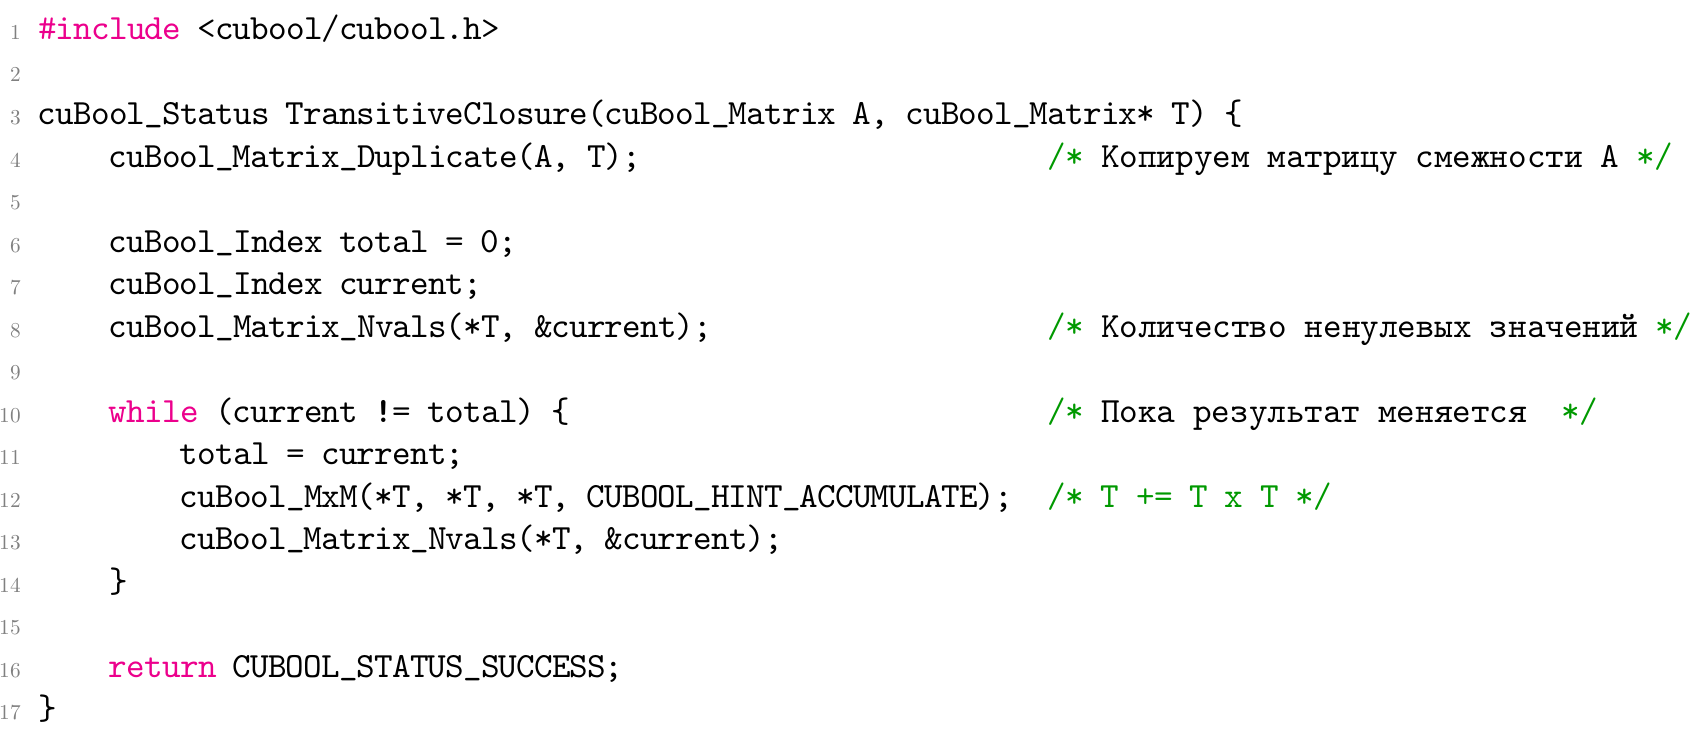
\includegraphics[width=\textwidth]{figures/tc_c_api.png}
            \caption{Вычисление транзитивного замыкания для ориентированного графа без меток с использованием \textbf{cuBool C API}}
        \end{figure}
    \end{minipage}\hfill    
    \end{center}   
\end{frame}

\begin{frame}[fragile] \frametitle{Пример использования Python API}
    \begin{center}
     \begin{minipage}[m]{0.9\linewidth}
        \begin{figure}
            \centering
            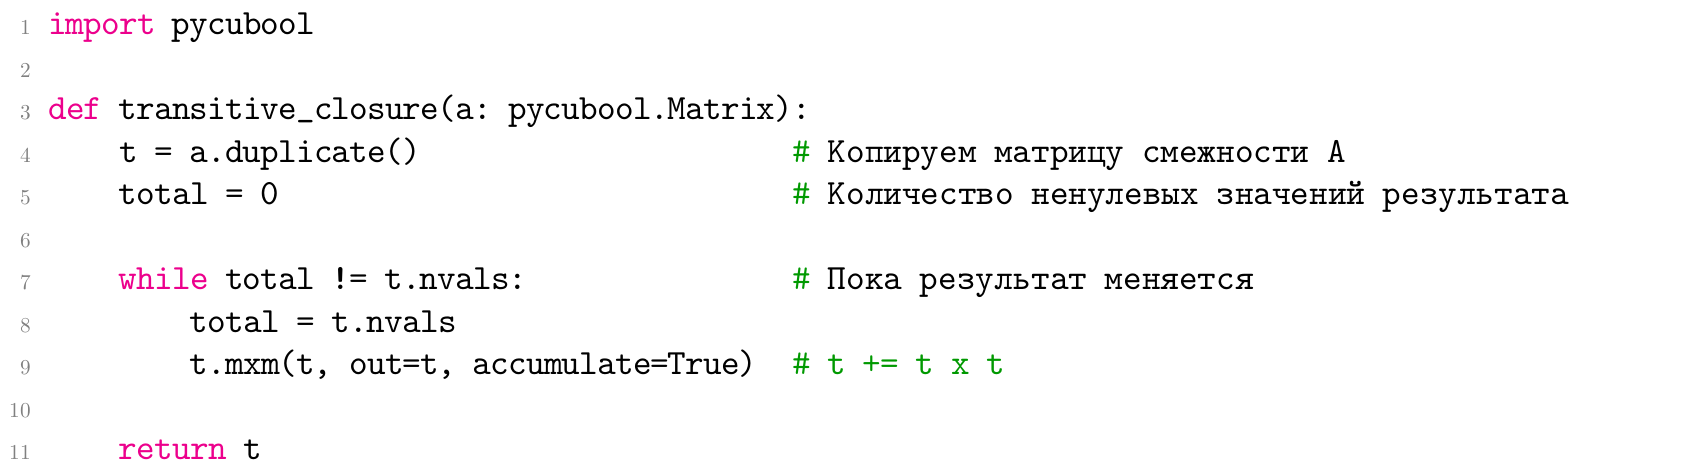
\includegraphics[width=\textwidth]{figures/tc_python_api.png}
            \caption{Вычисление транзитивного замыкания для ориентированного графа без меток с использованием \textbf{pycubool}}
        \end{figure}
    \end{minipage}\hfill   
    \end{center}
\end{frame}

\begin{frame}[fragile] \frametitle{Алгоритм поиска путей с КС ограничениями через тензорное произведение}
    \begin{itemize}
        \item Алгоритм реализован с использованием разработанного пакета pycubool
        \item Реализация доступна в рамках проекта CFPQ-PyAlgo
        \item Вход: ориентированный граф с метками на ребрах и КС грамматика в виде рекурсивного автомата
        \item Выход: матрица достижимости, а также индекс для восстановления всех пути в графе соответствии с входной грамматикой
    \end{itemize}
\end{frame}

\begin{frame}[fragile] \frametitle{Инфраструктура CFPQ-PyAlgo}
    \begin{center}
     \begin{minipage}[m]{0.65\linewidth}
        \begin{figure}
            \centering
            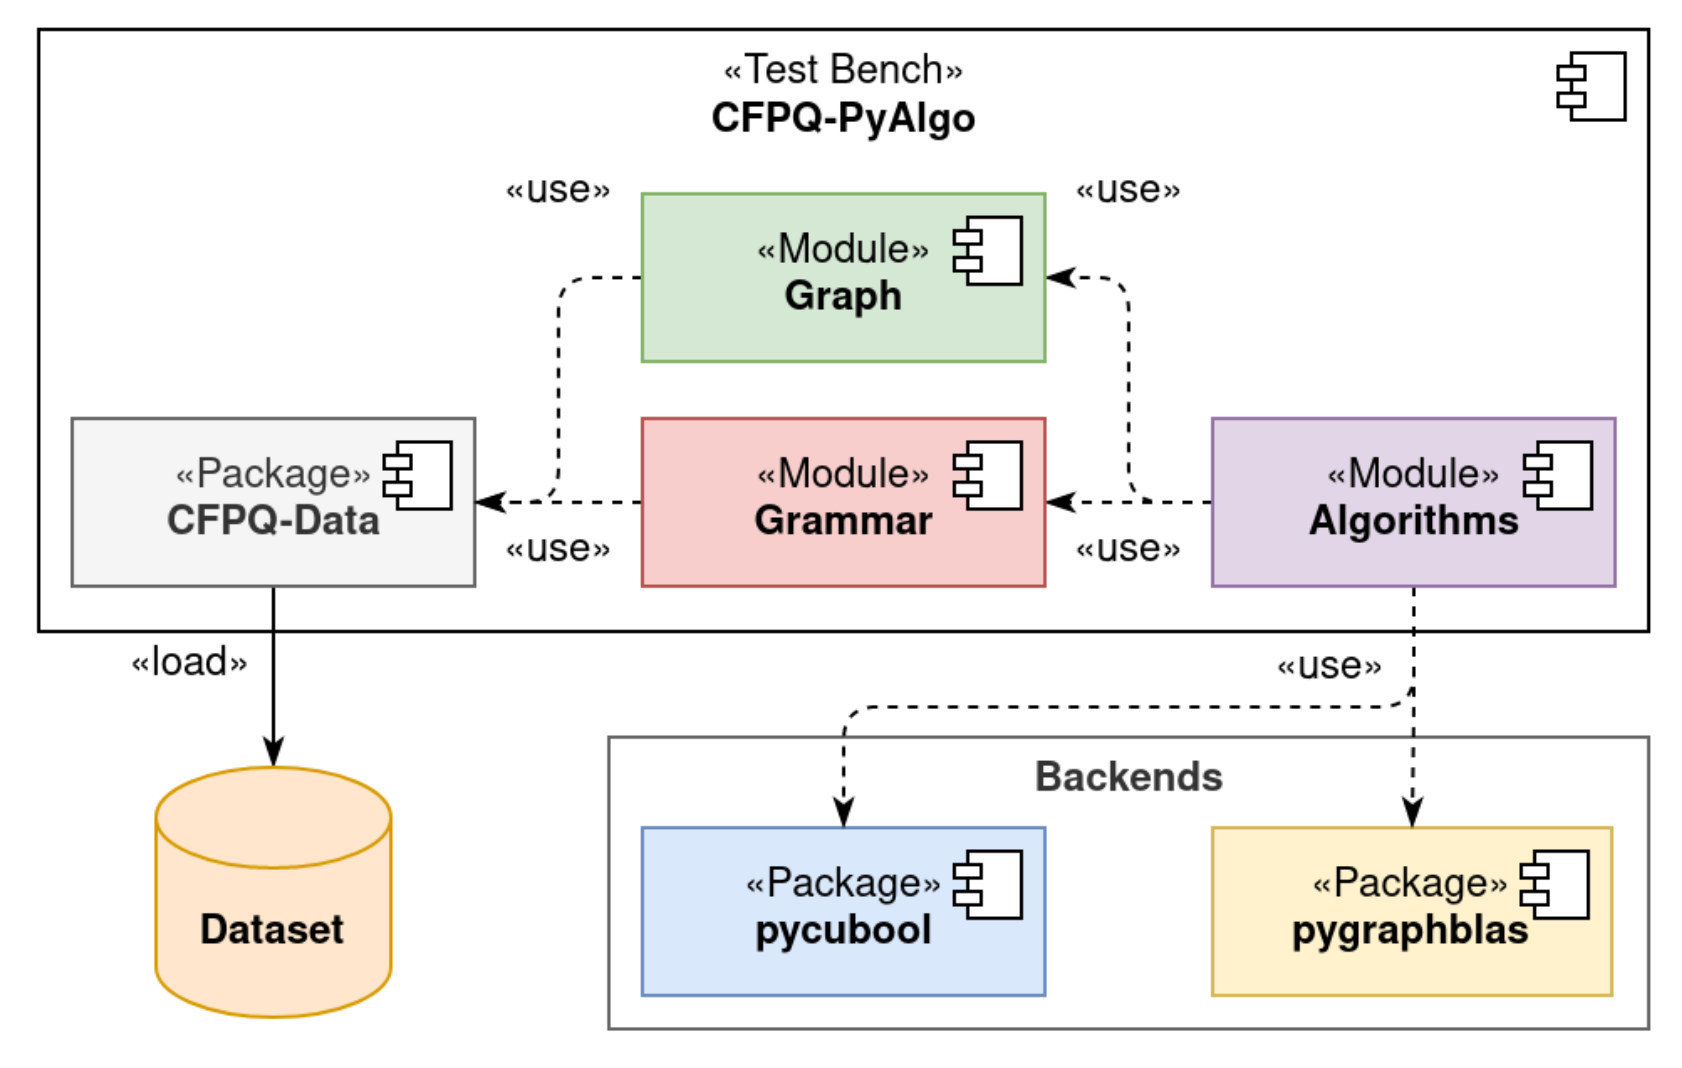
\includegraphics[width=\textwidth]{figures/cfpq_py_algo.png}
            \caption{Архитектура CFPQ-PyAlgo стенда для тестирования алгоритмов}
        \end{figure}
    \end{minipage}\hfill   
    \end{center}
\end{frame}

\begin{frame}[fragile] \frametitle{Экспериментальное исследование}
    \begin{itemize}
        \item Рабочая станция: Intel Core i7-6790, 3.40GHz, RAM DDR4 64Gb, GeForce GTX 1070 с 8Gb VRAM, ОС Ubuntu 20.04
        \item Данные, необходимые для замеров, предварительно загружаются в RAM или VRAM в требуемом формате
        \item Исследовательские вопросы:
        {
        \begin{itemize}
            \item[\textbf{В1:}] Какова производительность отдельных операций реализованной библиотеки примитивов разреженной линейной булевой алгебры на GPGPU по сравнению с существующими аналогами?
   
           \item[\textbf{В2:}] Какова производительность реализованного алгоритма поиска путей через тензорное произведение на GPGPU  по сравнению с существующими аналогами, также полагающимися на примитивы линейной алгебры?  
        \end{itemize}
        }
    \end{itemize}
\end{frame}

\begin{frame}[fragile] \frametitle{В1: Набор данных}
    \begin{center}
     \begin{minipage}[m]{0.9\linewidth}
        \begin{figure}
            \centering
            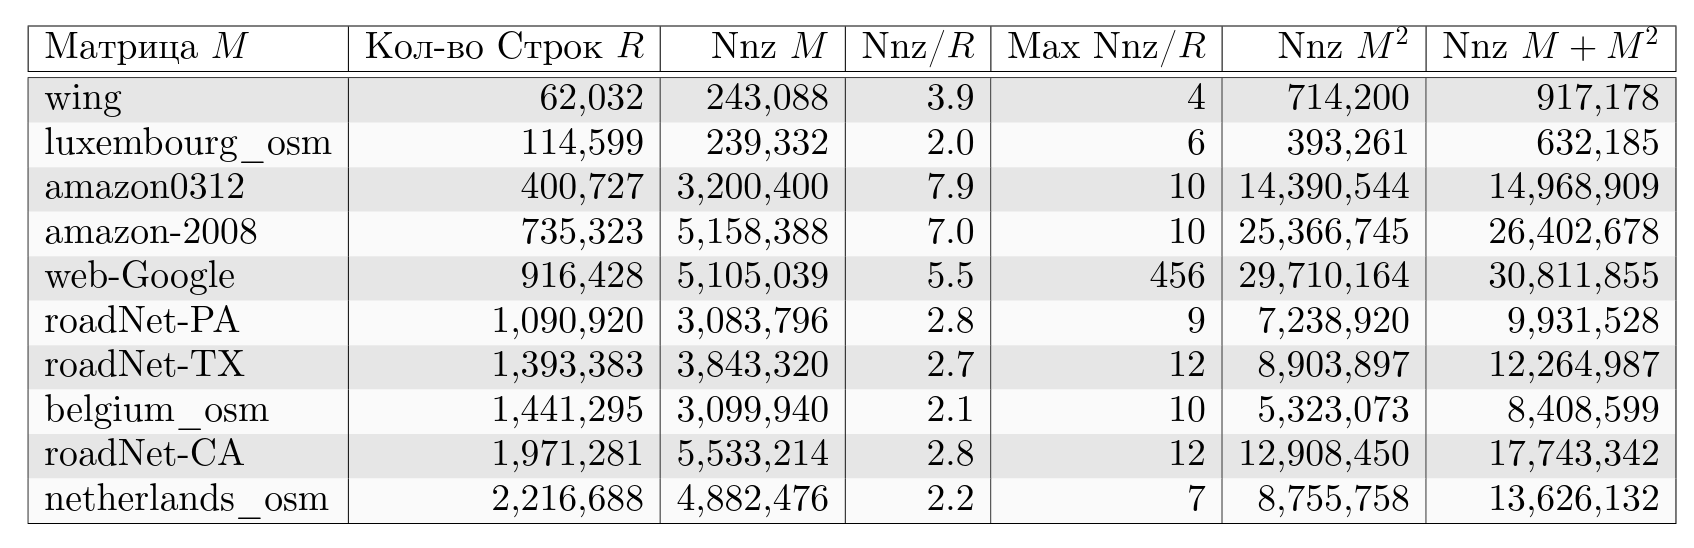
\includegraphics[width=1.0\textwidth]{figures/dataset_rq1.png}
            \caption{Разреженные матричные данные}
        \end{figure}
    \end{minipage}\hfill   
    \end{center}
\end{frame}

\begin{frame}[fragile] \frametitle{В1: Матричное умножение}
    \begin{center}
     \begin{minipage}[m]{0.85\linewidth}
        \begin{figure}
            \centering
            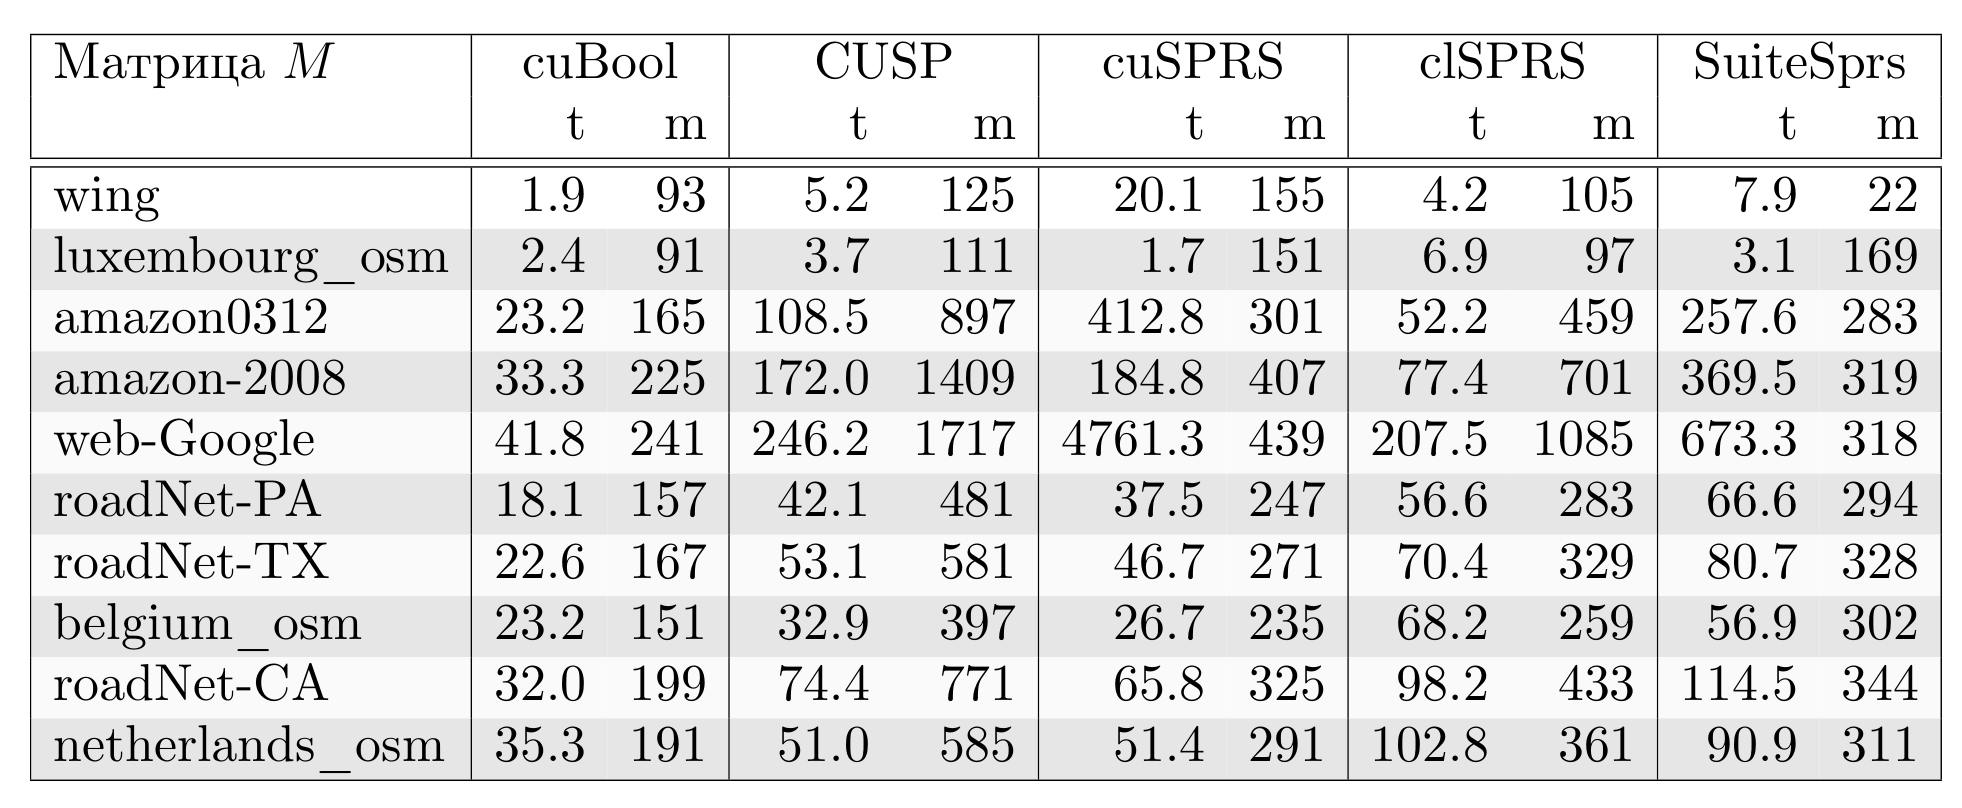
\includegraphics[width=1.0\textwidth]{figures/results_1_rq1.png}
            \caption{Матричное умножение, время (t) в миллисекундах, память (m) в мегабайтах, отклонение в пределах 10\%}
        \end{figure}
    \end{minipage}\hfill   
    \end{center}
\end{frame}

\begin{frame}[fragile] \frametitle{В1: Поэлементное матричное сложение}
    \begin{center}
     \begin{minipage}[m]{0.85\linewidth}
        \begin{figure}
            \centering
            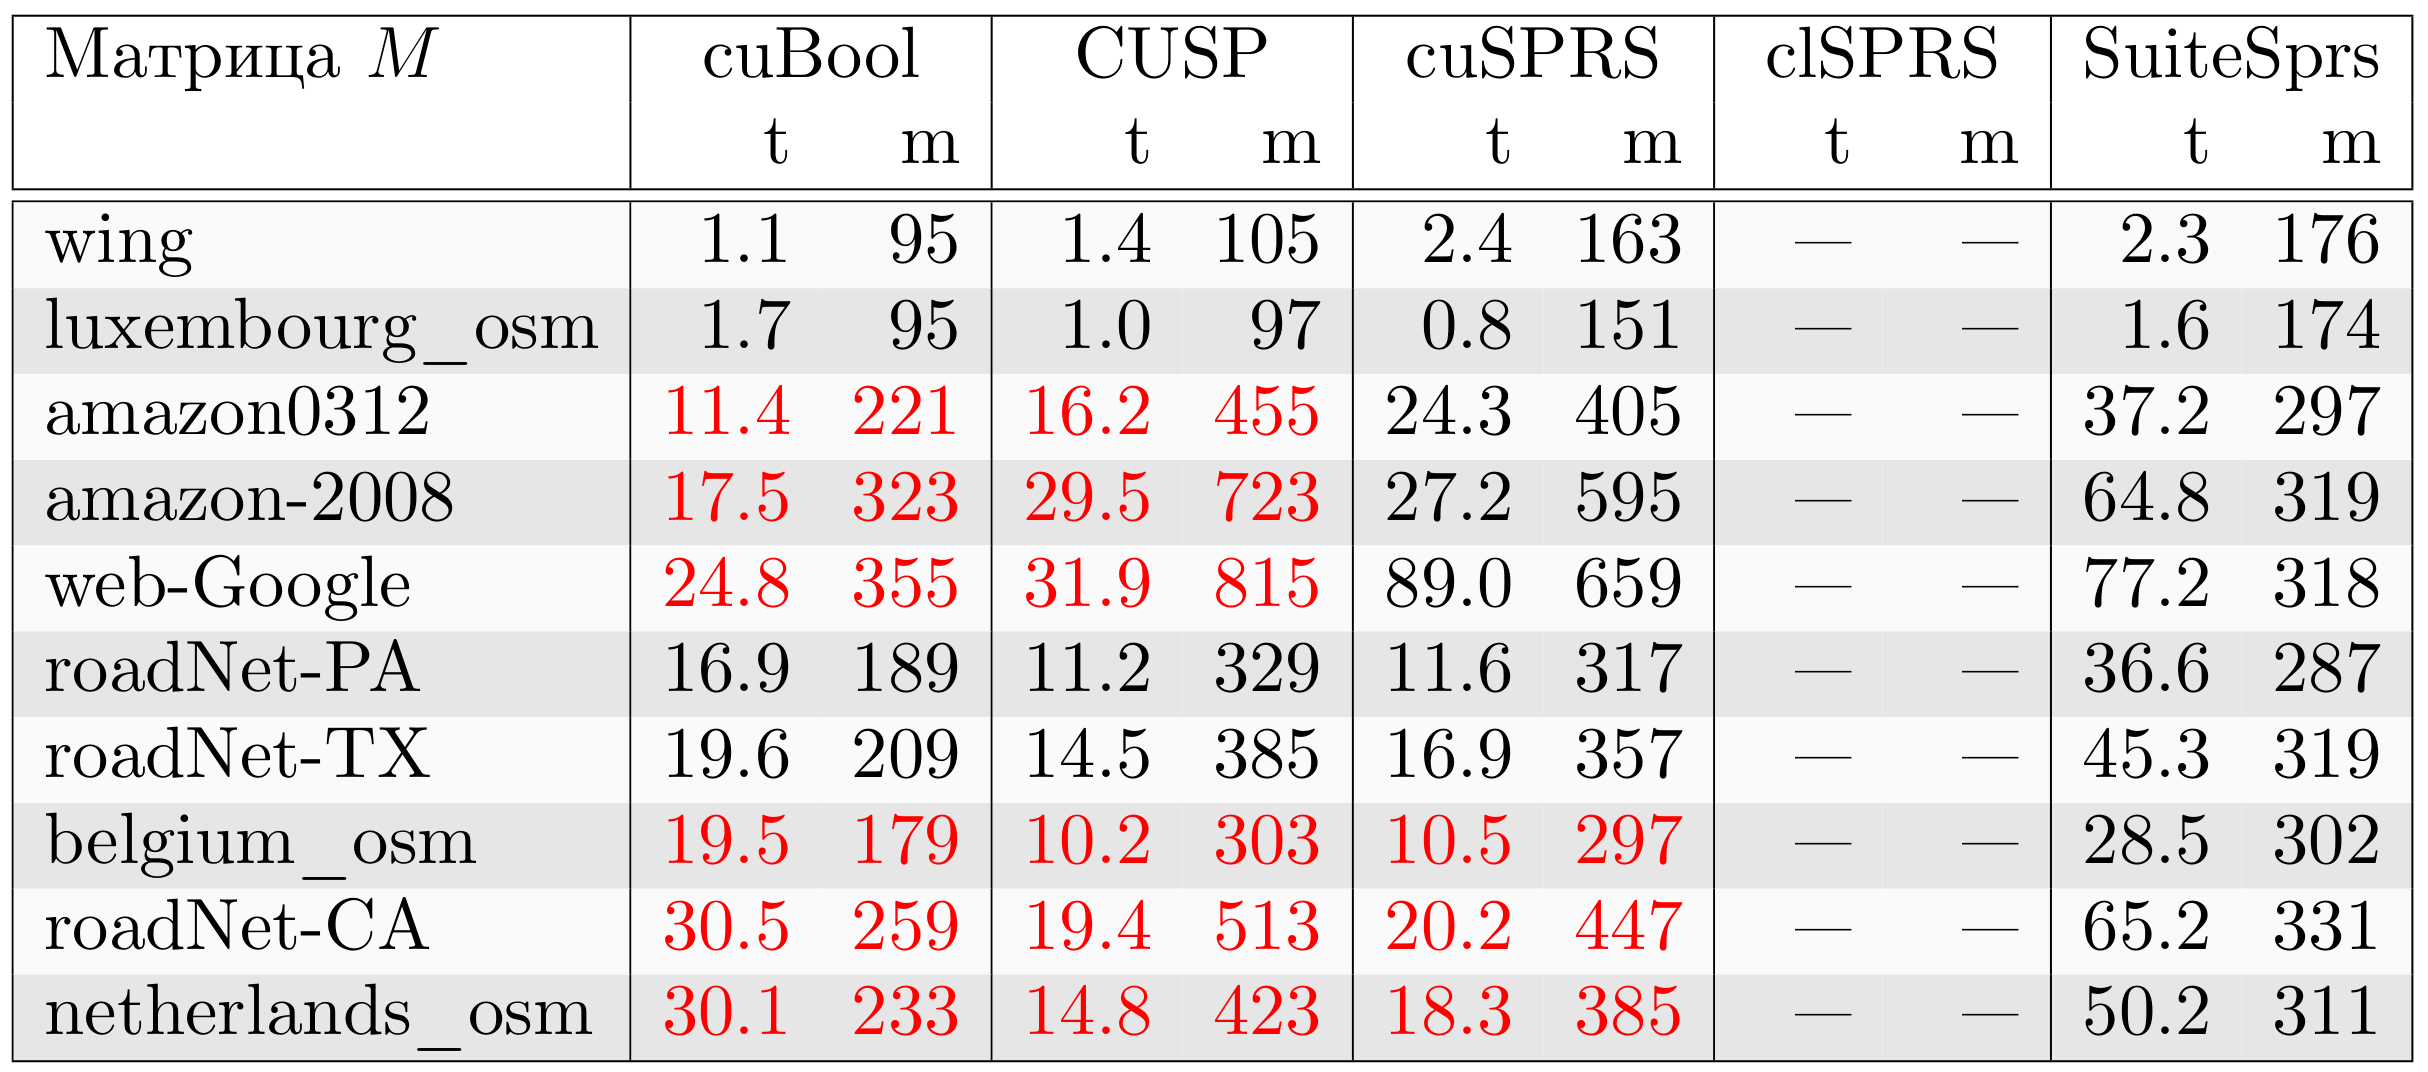
\includegraphics[width=1.0\textwidth]{figures/results_2_rq1.png}
            \caption{Поэлементное матричное сложение, время (t) в миллисекундах, память (m) в мегабайтах, отклонение в пределах 10\%}
        \end{figure}
    \end{minipage}\hfill   
    \end{center}
\end{frame}

\begin{frame}[fragile] \frametitle{В2: Набор данных}
    \begin{center}
     \begin{minipage}[m]{0.9\linewidth}
        \begin{figure}
            \centering
            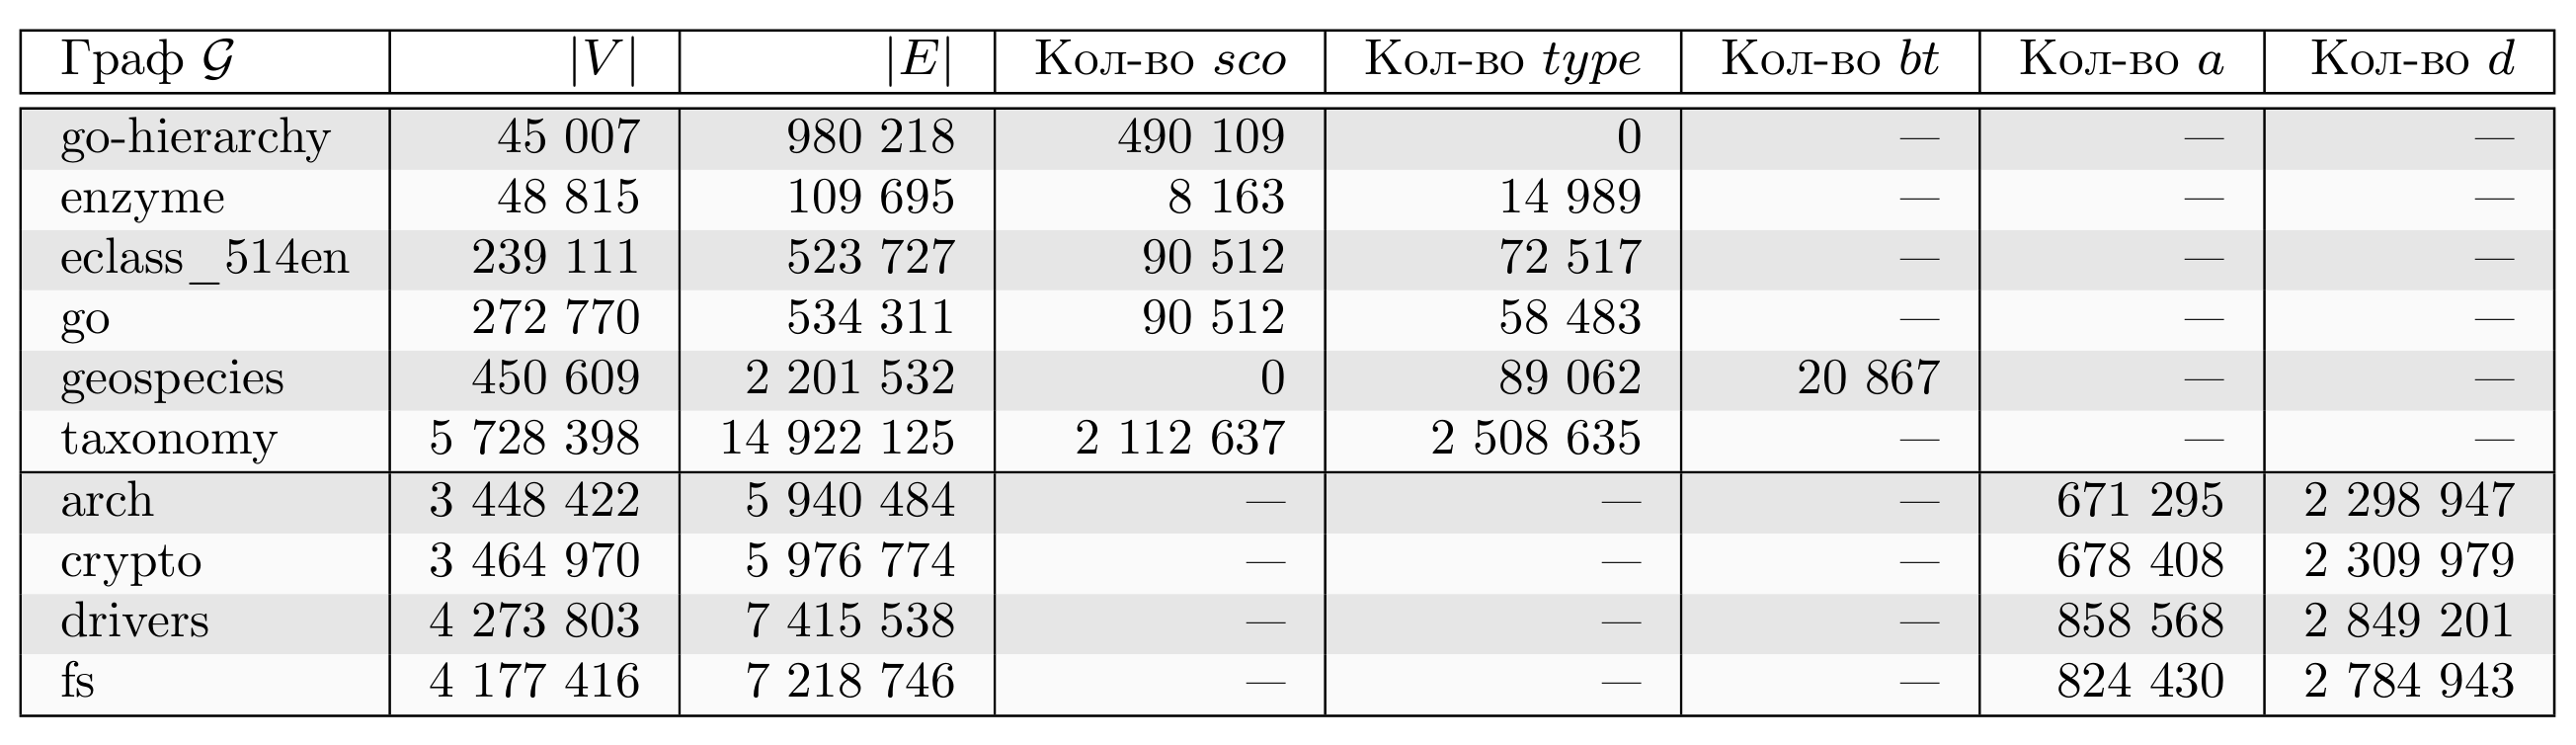
\includegraphics[width=1.0\textwidth]{figures/dataset_rq2.png}
            \caption{RDF графы и графы программ для экспериментов}
        \end{figure}
    \end{minipage}\hfill   
    \end{center}
\end{frame}

\begin{frame}[fragile] \frametitle{В2: Запросы с КС ограничениями}
    \begin{center}
     \begin{minipage}[m]{0.85\linewidth}
        \begin{figure}
            \centering
            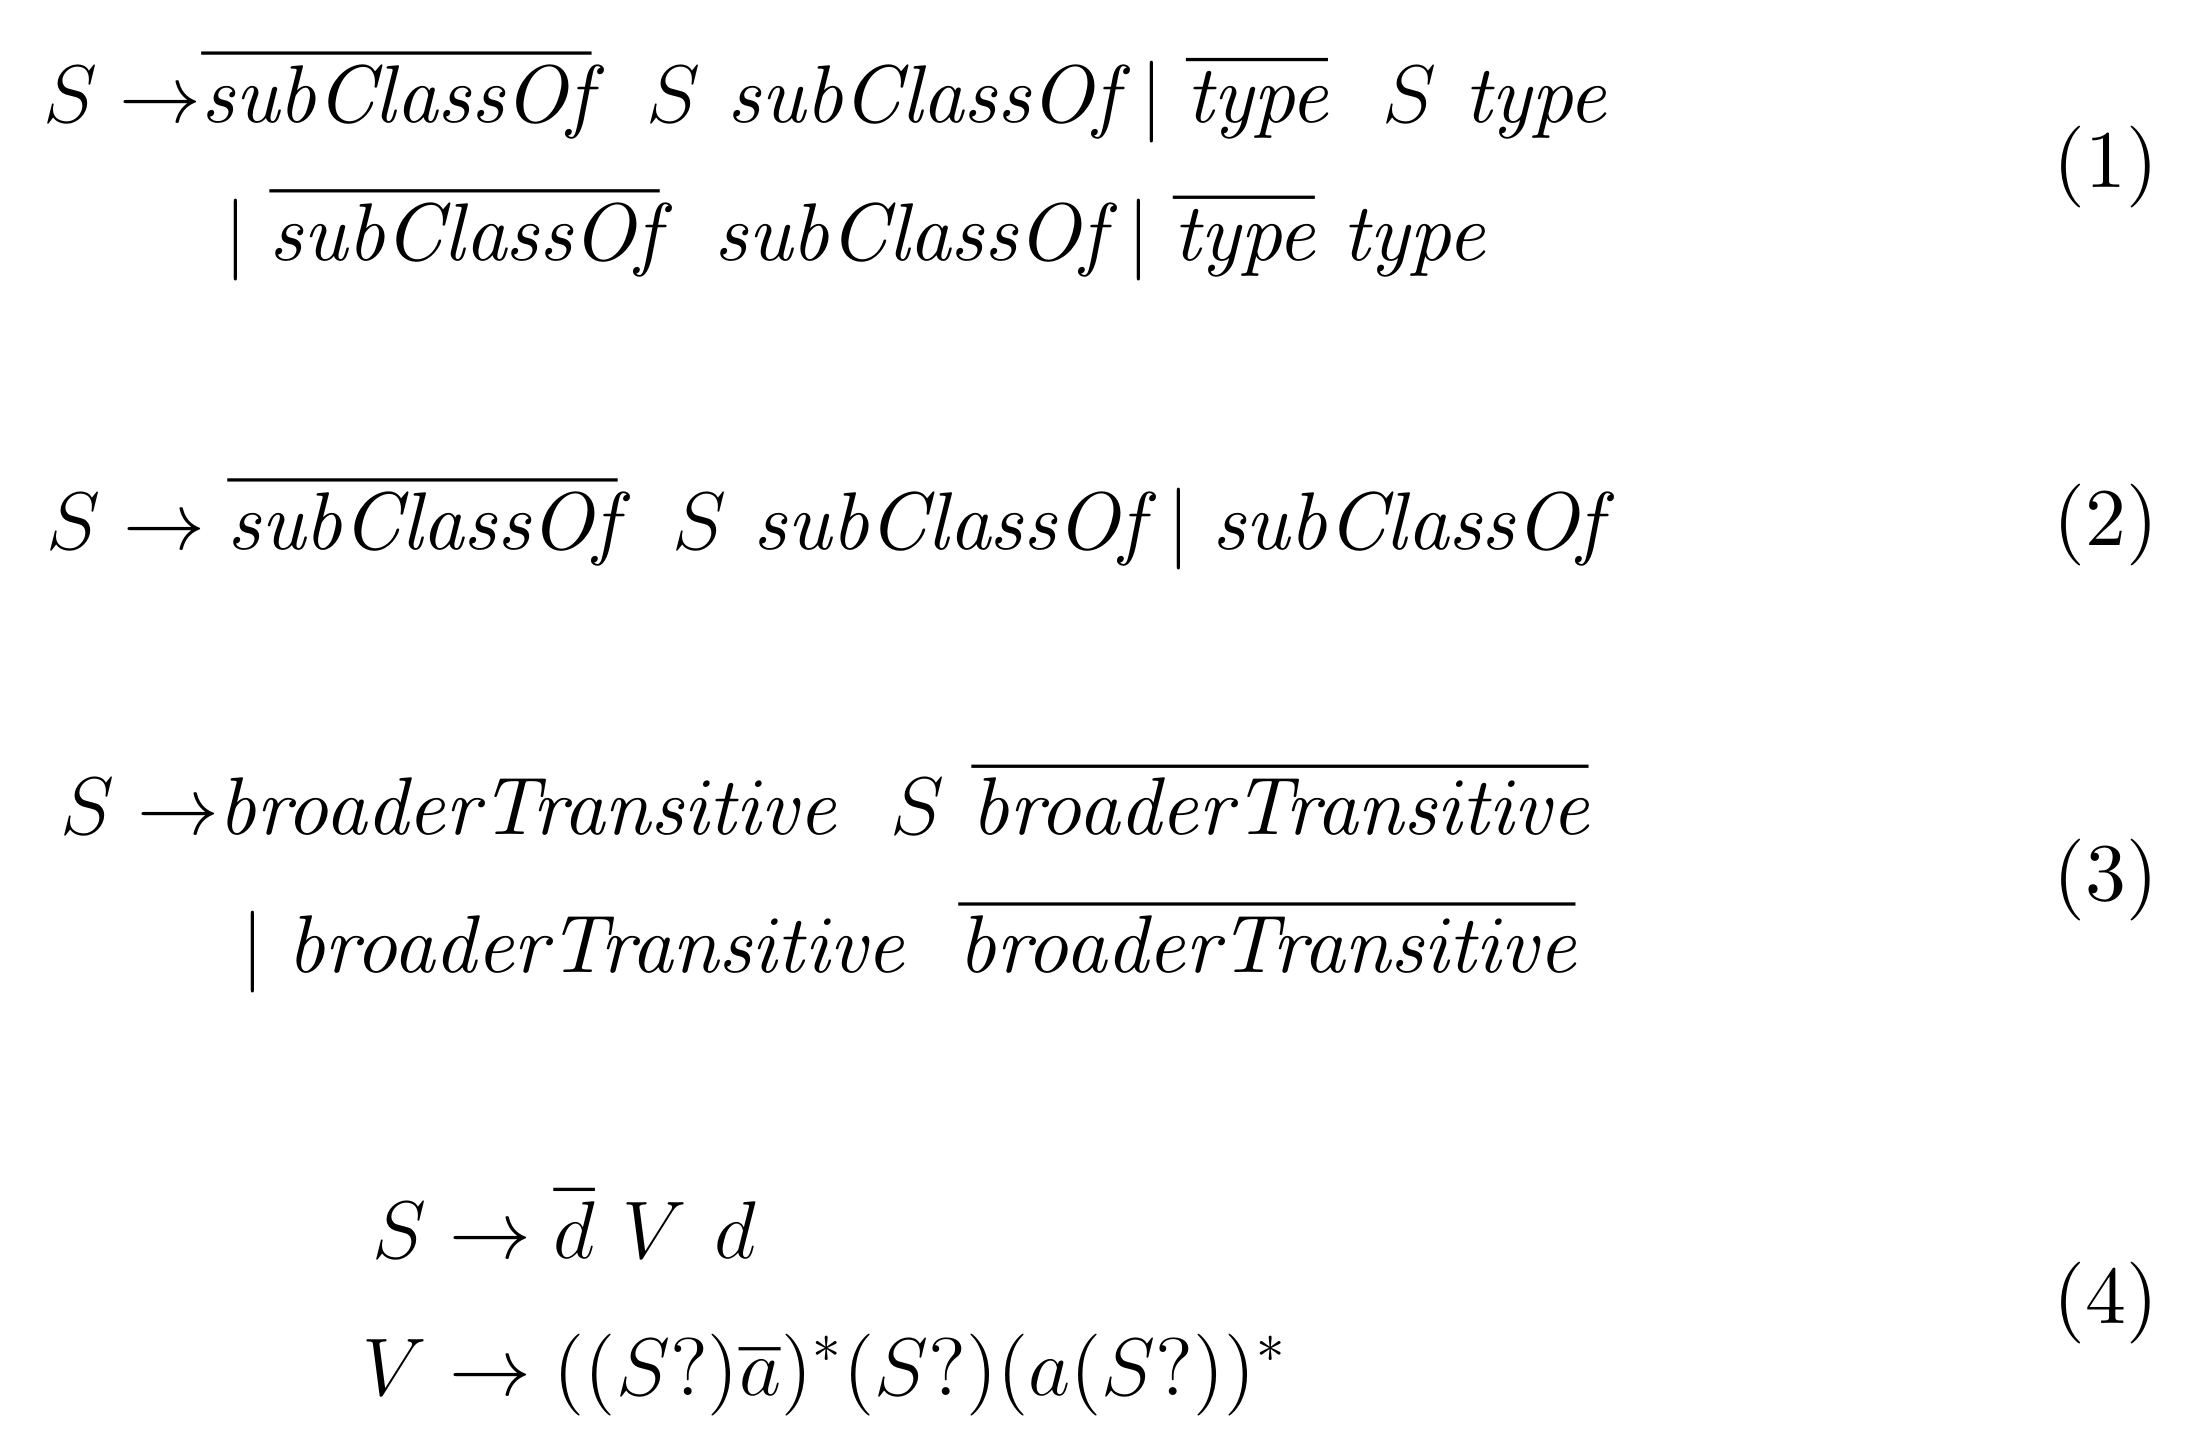
\includegraphics[width=0.65\textwidth]{figures/cfpq_query_rq2.png}
            \caption{КС грамматики запросов для анализа. Запросы, для анализа RDF данных: $G_1$ (1), $G_2$ (2), $G_{geo}$ (3), для анализа указателей в графах программ --- $G_{ma}$ (4).}
        \end{figure}
    \end{minipage}\hfill   
    \end{center}
\end{frame}

\begin{frame}[fragile] \frametitle{В2: Анализ RDF данных}
    \begin{center}
     \begin{minipage}[m]{0.9\linewidth}
        \begin{figure}
            \centering
            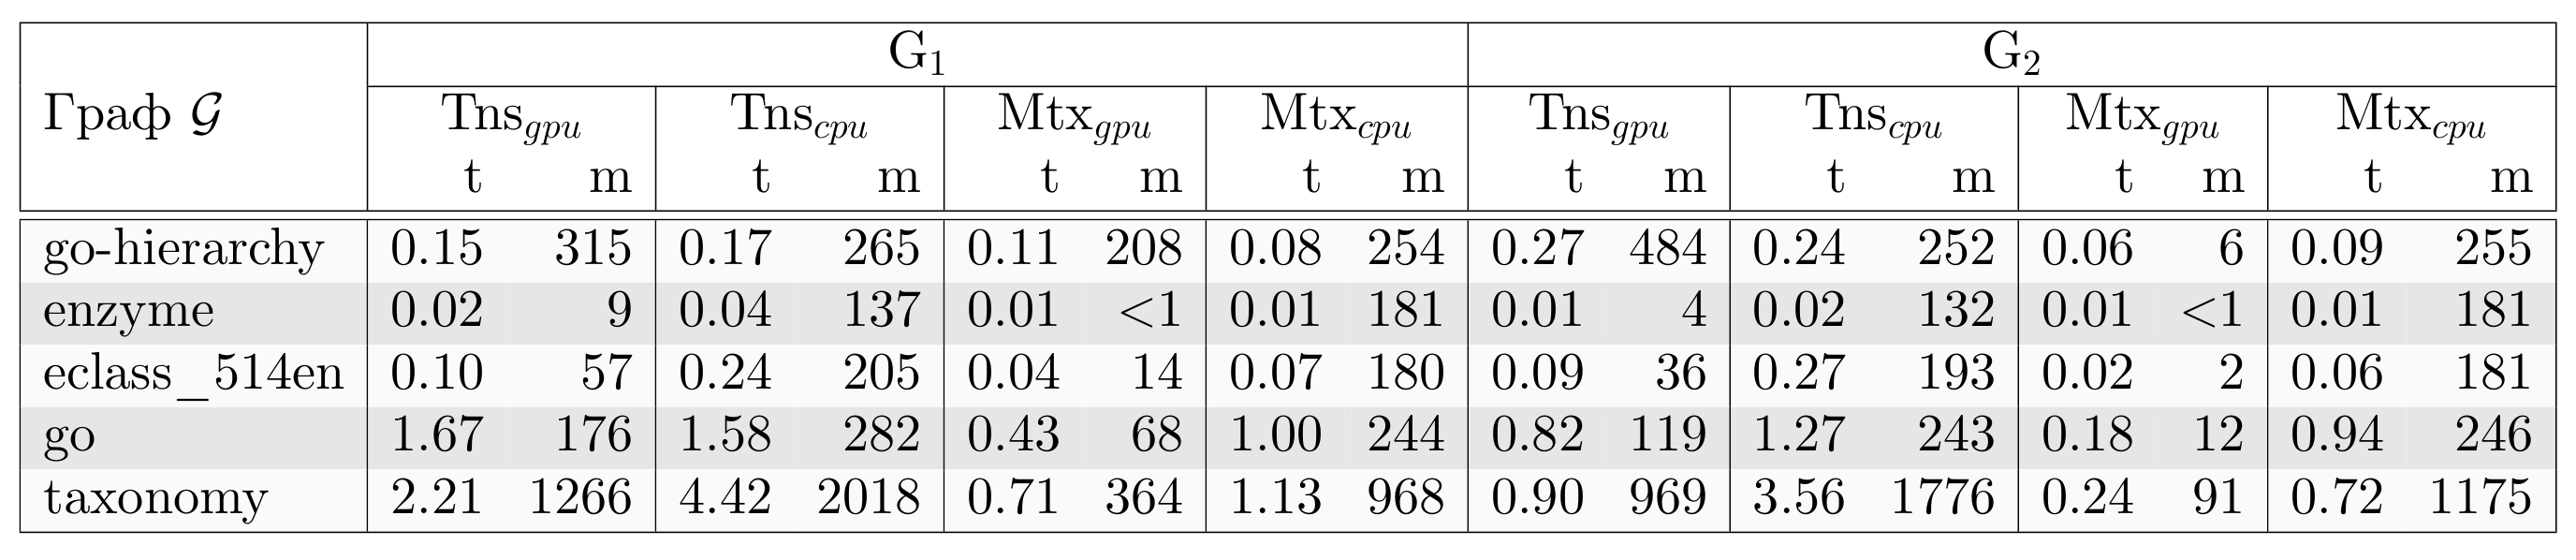
\includegraphics[width=1.0\textwidth]{figures/results_1_rq2.png}
            \caption{Анализ RDF данных с использованием запросов $G_1$ и $G_2$, время (t) в секундах, память (m) в мегабайтах, отклонение в пределах 10\%}
        \end{figure}
    \end{minipage}\hfill   
    \begin{minipage}[m]{0.9\linewidth}
        \begin{figure}
            \centering
            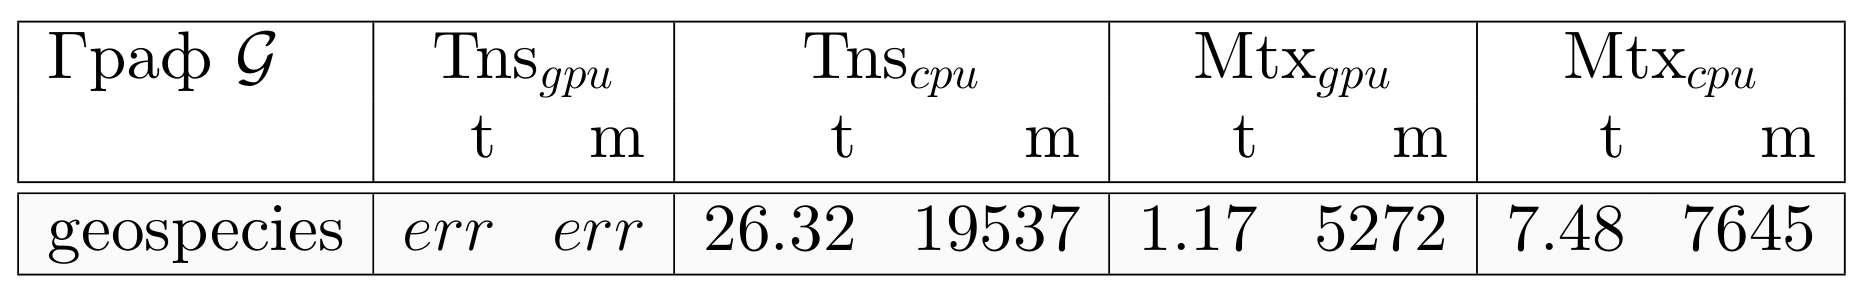
\includegraphics[width=0.6\textwidth]{figures/results_2_rq2.png}
            \caption{Анализ RDF данных с использованием запроса $G_{geo}$, время (t) в секундах, память (m) в мегабайтах, отклонение в пределах 10\%}
        \end{figure}
    \end{minipage}
    \end{center}
\end{frame}

\begin{frame}[fragile] \frametitle{В2: Анализ указателей}
    \begin{center}
     \begin{minipage}[m]{0.9\linewidth}
        \begin{figure}
            \centering
            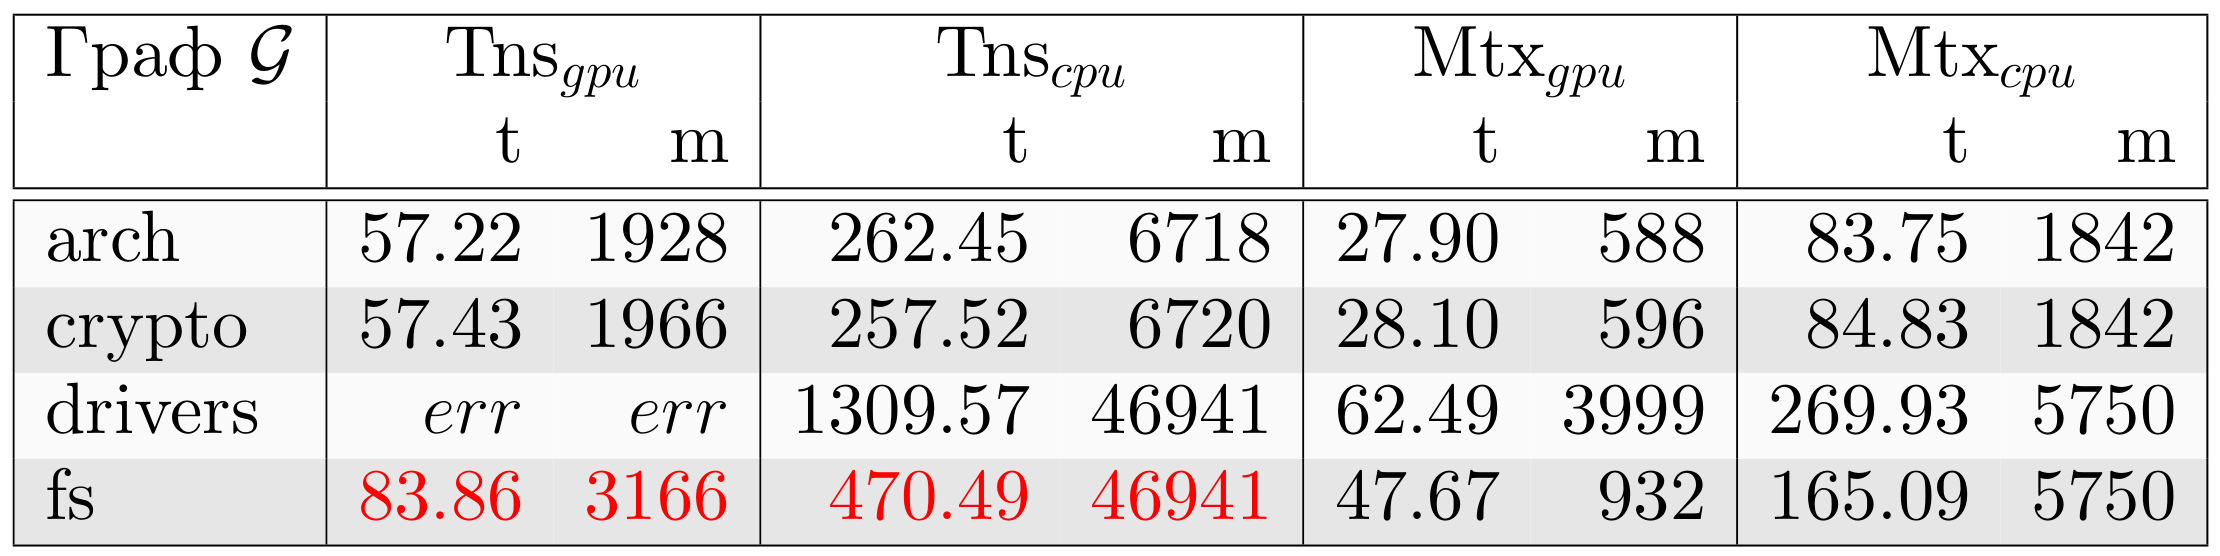
\includegraphics[width=0.7\textwidth]{figures/results_3_rq2.png}
            \caption{Анализ указателей с использованием запроса $G_{ma}$, время (t) в секундах, память (m) в мегабайтах, отклонение в пределах 10\%}
        \end{figure}
    \end{minipage}\hfill   
    \end{center}
\end{frame}

\begin{frame}[fragile] \frametitle{Заключение}
    \begin{itemize}
        \item Спроектирована библиотека примитивов линейной булевой алгебры для работы с разреженными данными на GPGPU
        \item Реализована библиотека cuBool\footnote{GitHub cuBool: \url{https://github.com/JetBrains-Research/cuBool}} в соответствии с разработанной архитектурой, опубликован соответствующий python-пакет\footnote{PyPI pycubool: \url{https://test.pypi.org/project/pycubool/}} 
        \item С использованием pycubool реализован алгоритм поиска путей с КС ограничениями через тензорное произведение
        \item Выполнено экспериментальное исследование полученных артефактов
        \break
        \item  Результаты исследования были представлены на конференции GrAPL 2021\footnote{GrAPL 2021: Workshop on Graphs, Architectures, Programming, and Learning. Сайт конференции: \url{https://hpc.pnl.gov/grapl/}.}
    \end{itemize}
\end{frame}

% \begin{frame}[fragile] \frametitle{Пример графа и матрицы}
%     \begin{minipage}[m]{1.0\linewidth}
%         \begin{figure}
%             \centering
%             \begin{subfigure}[b]{0.47\textwidth}
%                 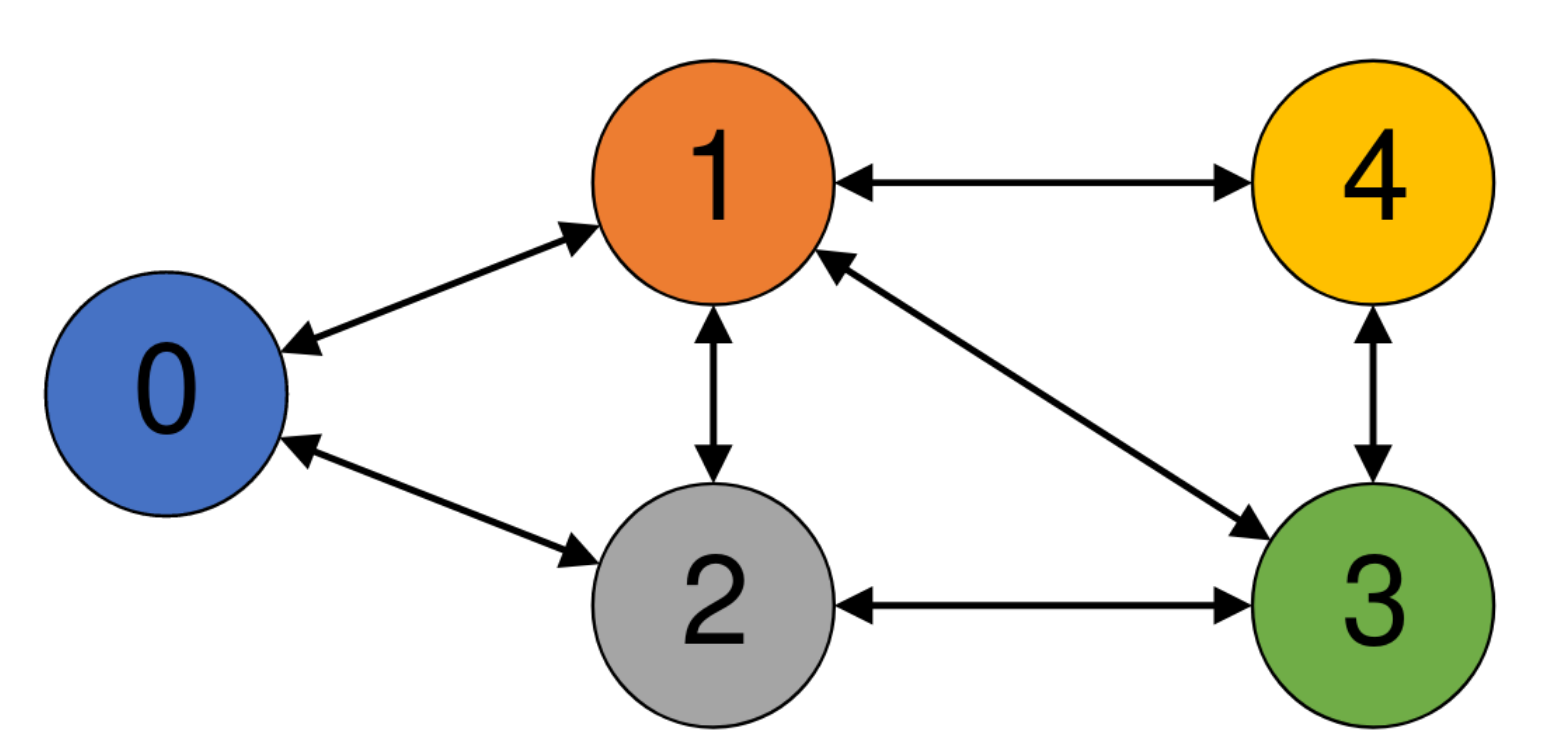
\includegraphics[width=\textwidth]{figures/graph.png}
%                 \caption{Graph}
%             \end{subfigure}
%             \hfill
%             \begin{subfigure}[b]{0.47\textwidth}
%                 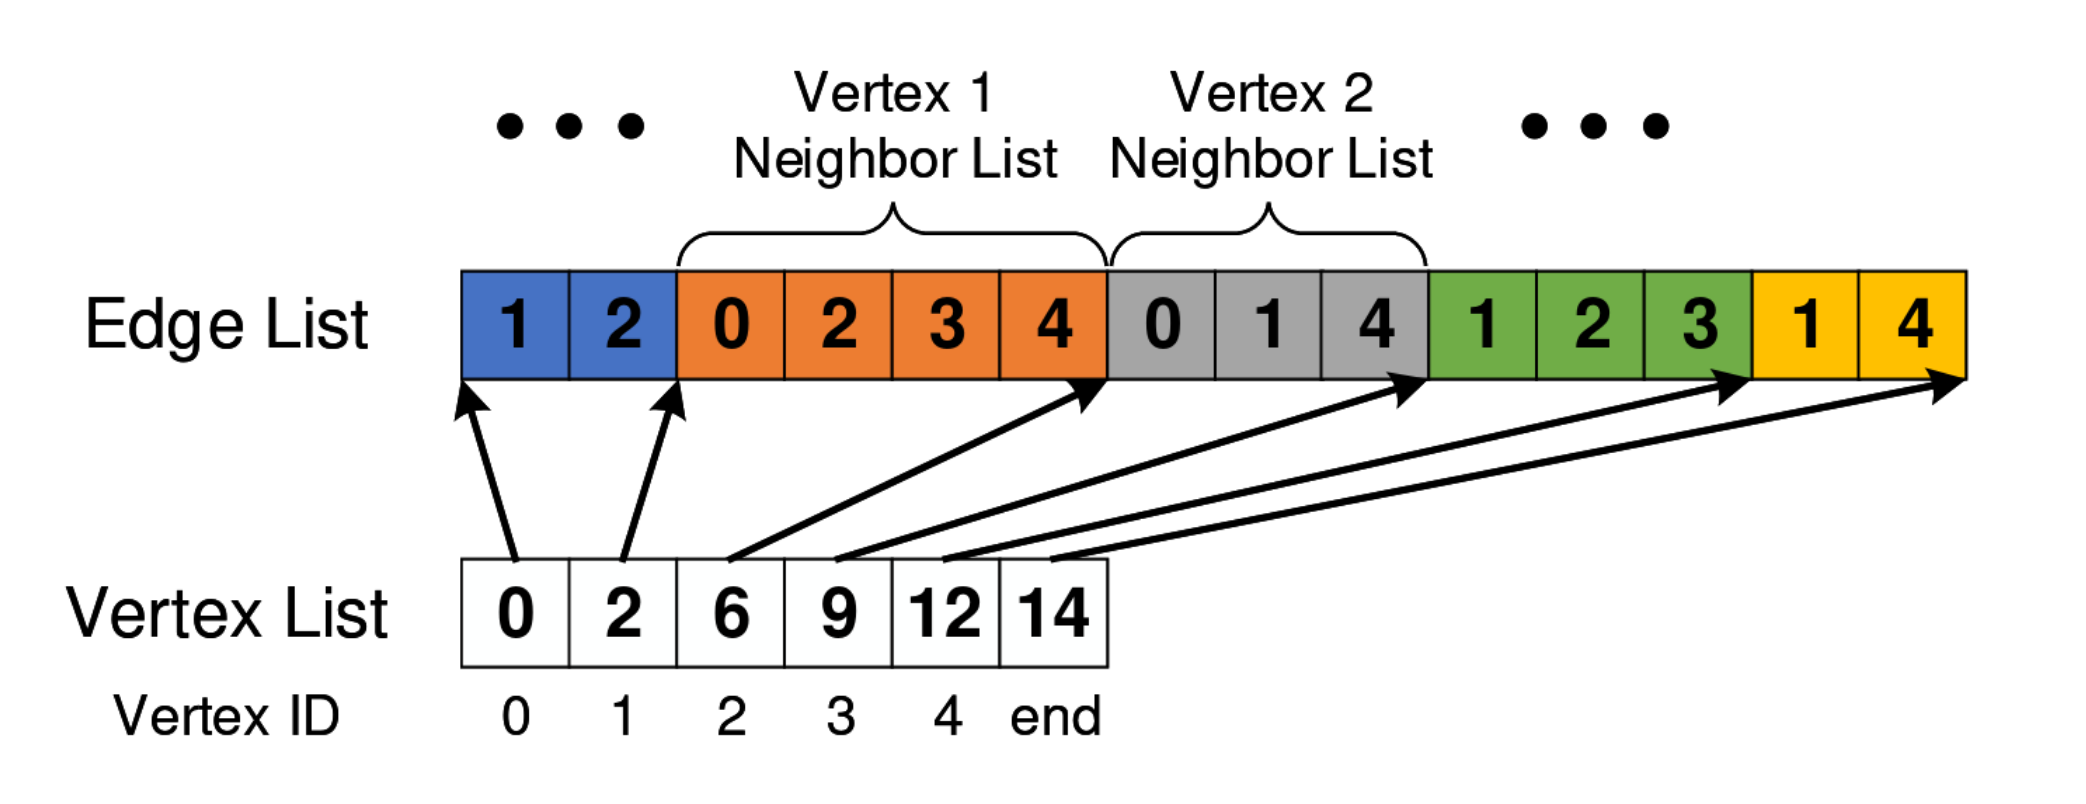
\includegraphics[width=\textwidth]{figures/csr_matrix.png}
%                 \caption{CSR matrix}
%             \end{subfigure}
%             \caption{Sample directed graph and its CSR adjacency matrix}
%         \end{figure}
%     \end{minipage}\hfill
% \end{frame}

% \begin{frame}[fragile] \frametitle{Результаты}
%     \begin{center}
%     \begin{minipage}[m]{0.85\linewidth}
%         \begin{figure}
%             \centering
%             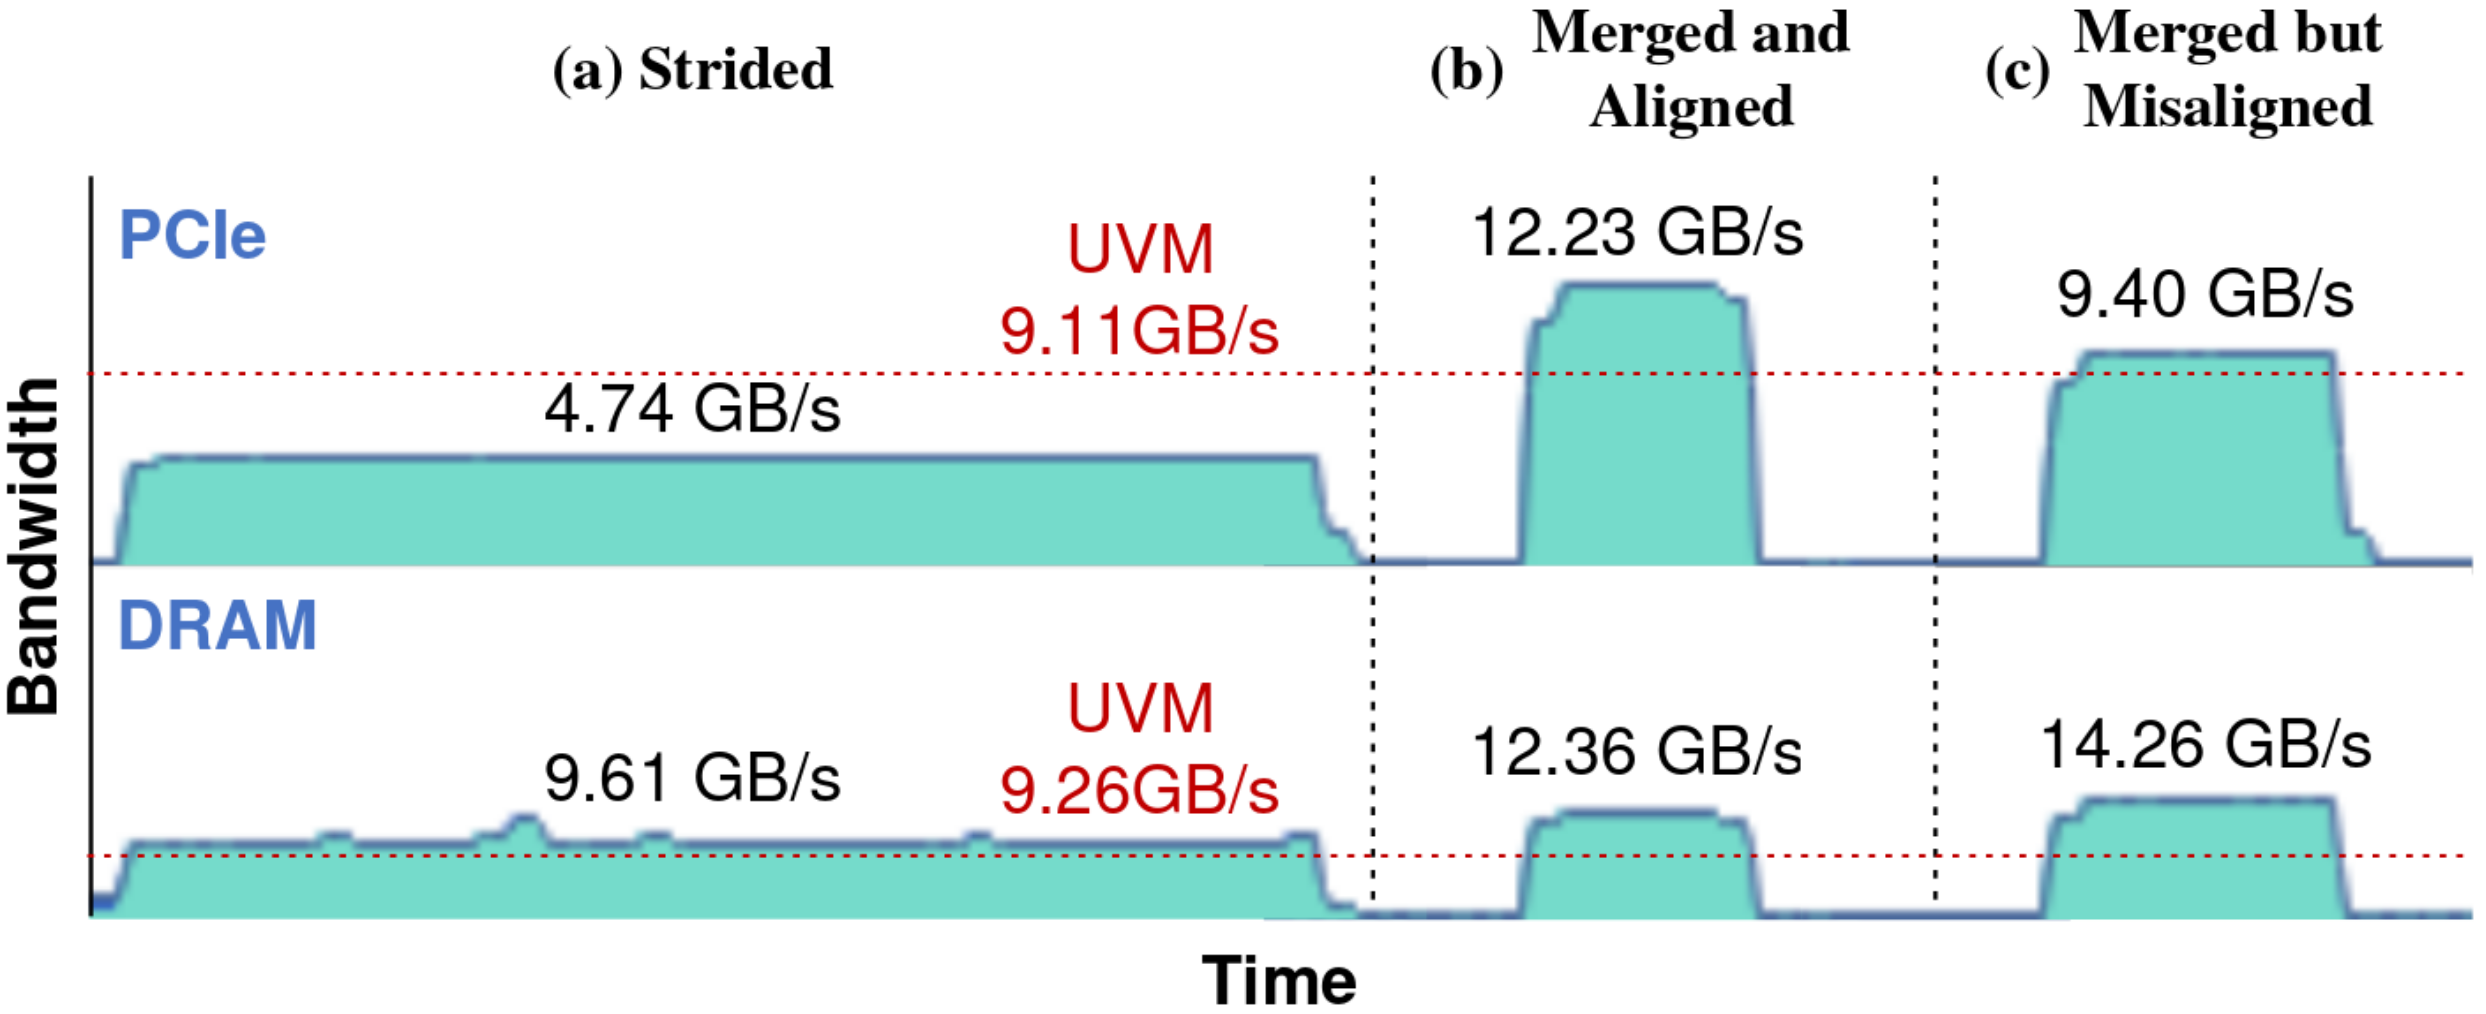
\includegraphics[width=\textwidth]{figures/access_patterns_utilization.png}
%             \caption{Average PCIe and DRAM bandwidth utilization for the dif-ferent zero-copy access patterns}
%             \label{fig:access_patterns_utilization}
%         \end{figure}
%     \end{minipage}\hfill
%     \end{center} 
% \end{frame}

% \begin{frame}[fragile] \frametitle{EMOGI}
%     \begin{minipage}[m]{1.0\linewidth}
%         \begin{figure}
%             \centering
%             \begin{subfigure}[b]{0.44\textwidth}
%                 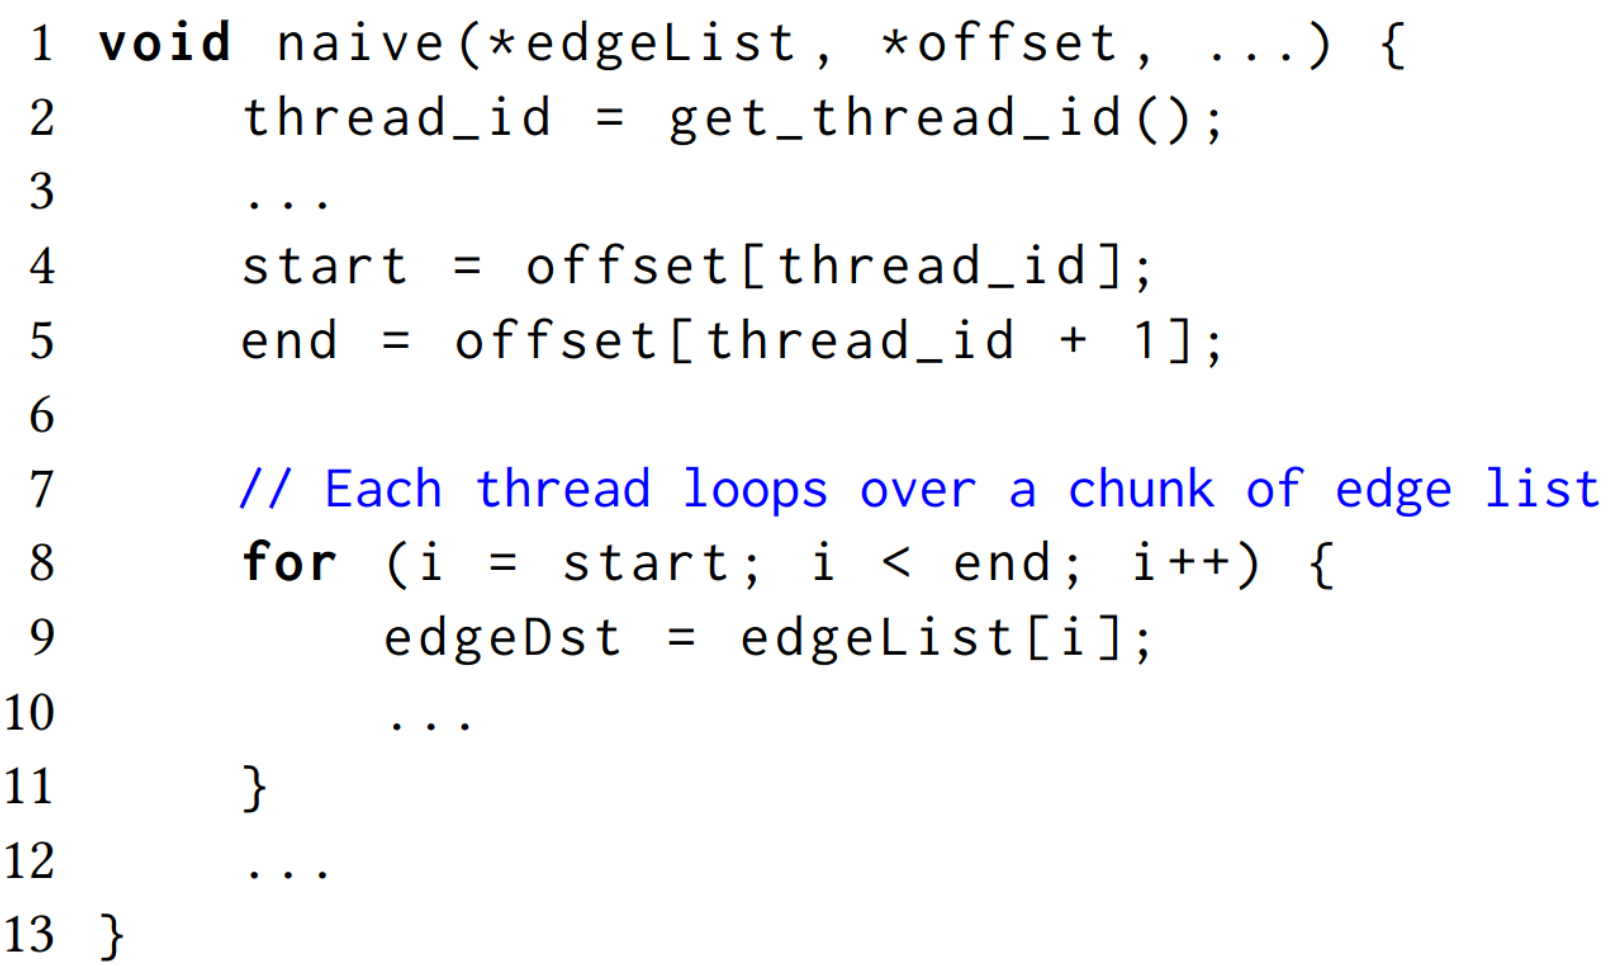
\includegraphics[width=\textwidth]{figures/emogi_naive.png}
%                 \caption{Na\"{\i}ve Uncoalesced Memory Access}
%             \end{subfigure}
%             \hfill
%             \begin{subfigure}[b]{0.44\textwidth}
%                 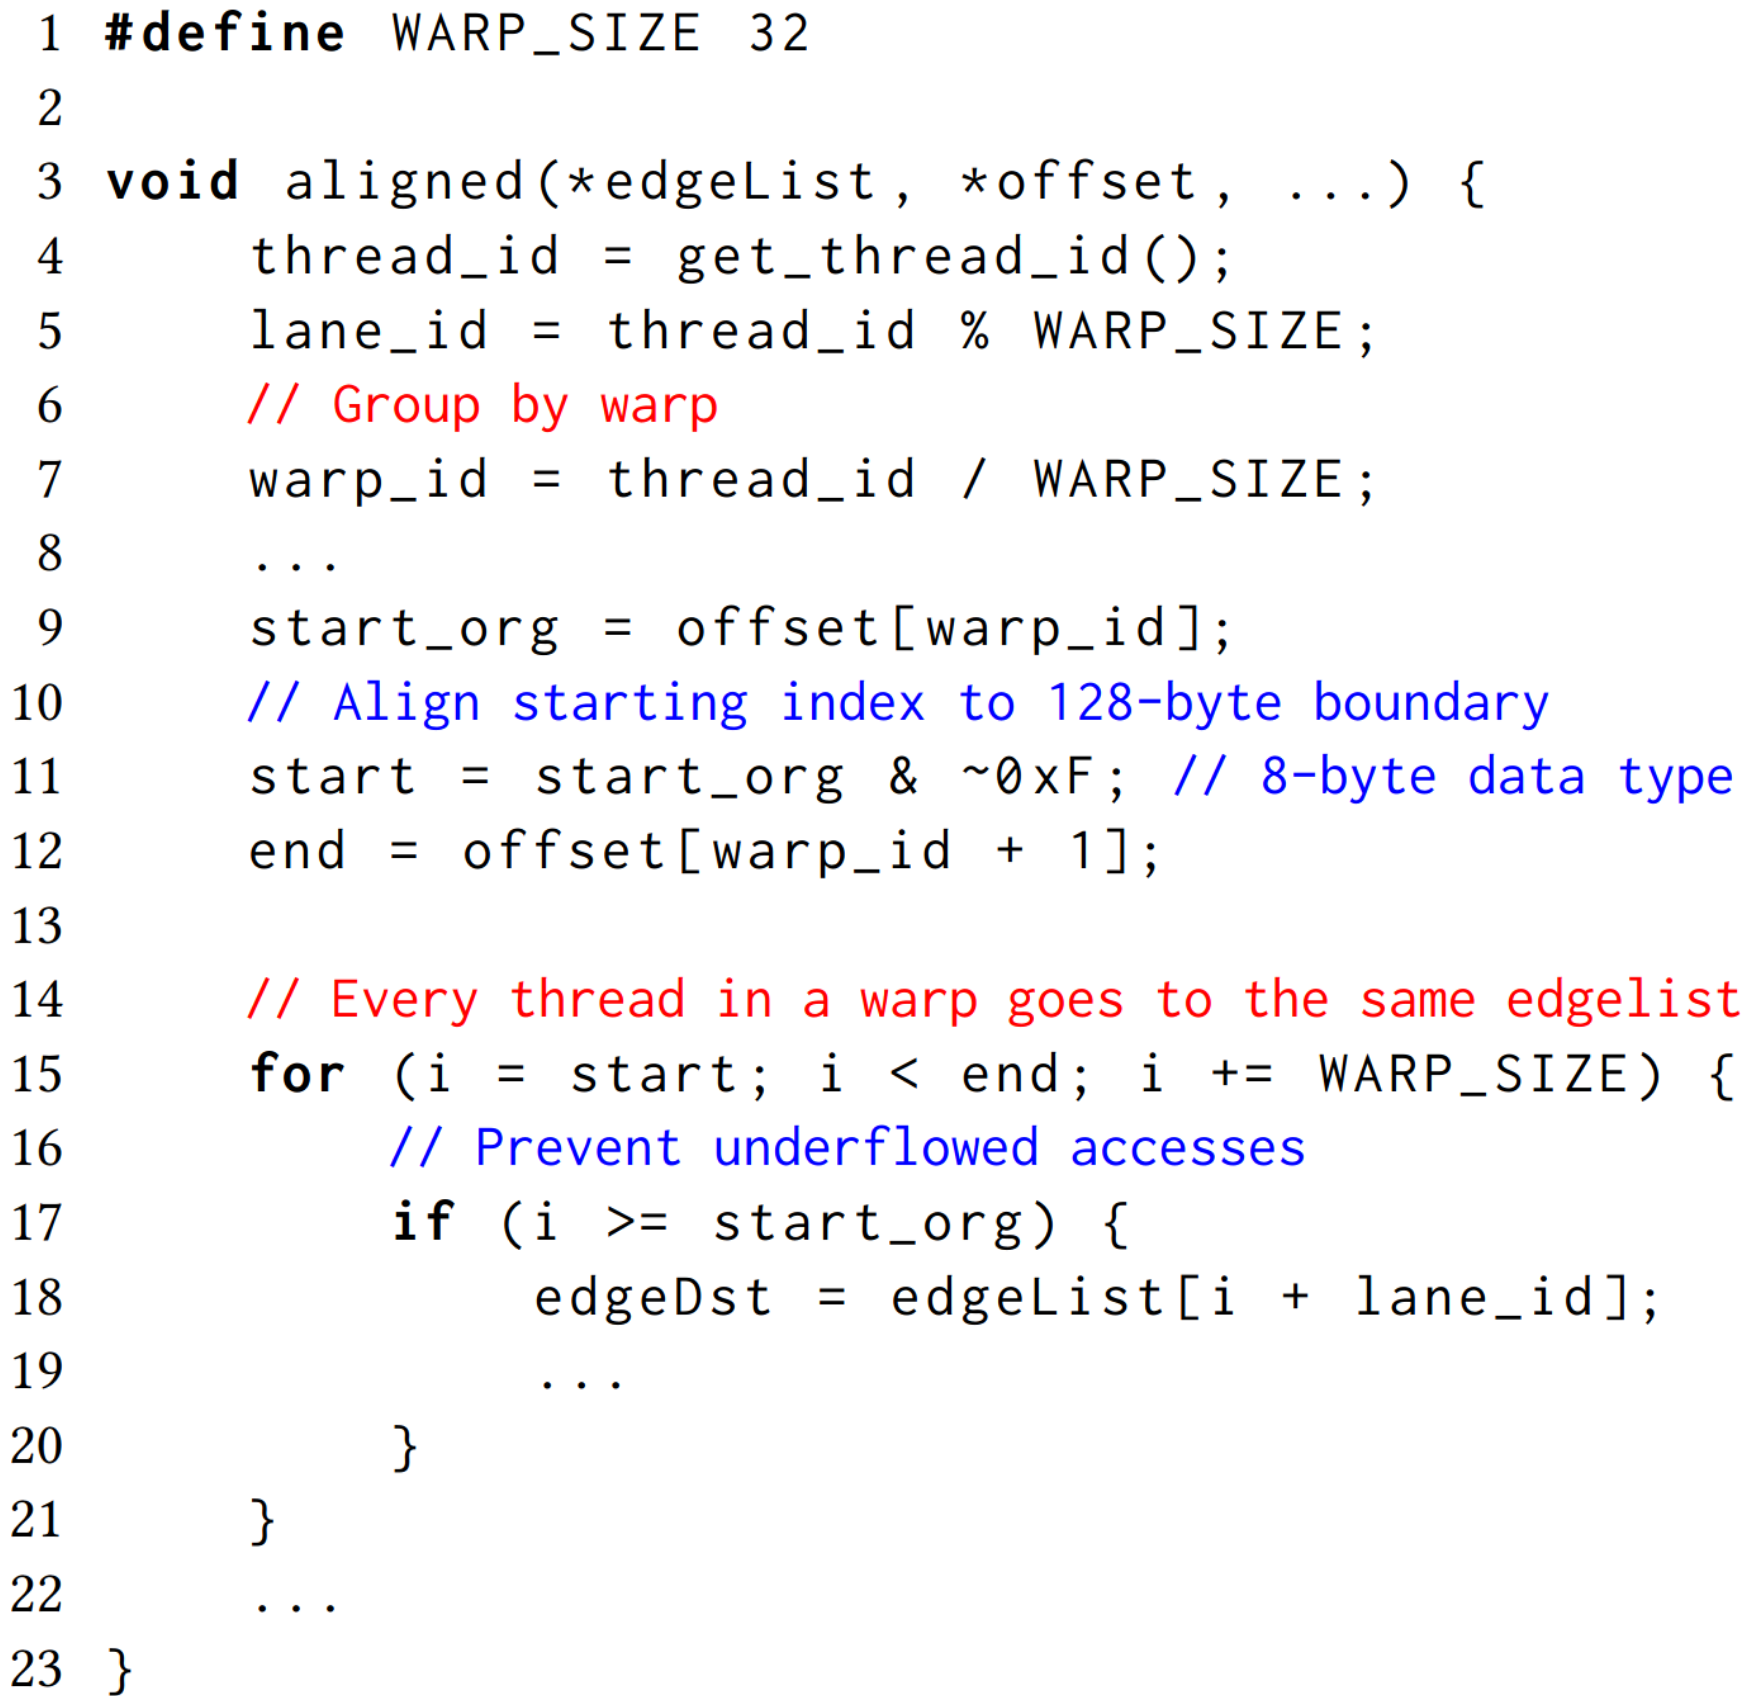
\includegraphics[width=\textwidth]{figures/emogi.png}
%                 \caption{EMOGI Coalesced Memory Access (Merged and Aligned)}
%             \end{subfigure}
%             \caption{Code listing for solution}
%         \end{figure}
%     \end{minipage}\hfill
% \end{frame}

% \begin{frame} \frametitle{Дополнительно}
%     \begin{itemize}
%         \item Почта: \href{mailto:egororachyov@gmail.com}{egororachyov@gmail.com}
%         \item Материалы презентации:
%         {
%             \begin{itemize}
%                 \item Arseniy Terekhov \& Artyom Khoroshev \& Rustam Azimov \& Semyon Grigorev (2020). Context-Free Path Querying with Single-Path Semantics by Matrix Multiplication. 1-12. 10.1145/3398682.3399163. 
%                 \item Egor Orachev \& Ilya Epelbaum \& Rustam Azimov \& Semyon Grigorev. (2020). Context-Free Path Querying by Kronecker Product. 10.1007/978-3-030-54832-2\_6. 
%             \end{itemize}
%         }
%         \item Ссылка на проект Cubool: \href{https://github.com/JetBrains-Research/cuBool}{https://github.com/JetBrains-Research/cuBool}
%     \end{itemize}
% \end{frame}

\end{document}
